%%%  کلاس AUTthesis، نسخه آبان 1397
%%%   دانشگاه صنعتی امیرکبیر                 http://www.aut.ac.ir
%%%  تالار گفتگوی پارسی‌لاتک،       http://forum.parsilatex.com
%%%   آپدیت شده در آبان 95
%%%   پشتیبانی و راهنمایی          badali_farhad@yahoo.com
%%%
%%%   بازبینی و اصلاح شده در آبان ماه 1397
%%%  Tested via TeXstudio in TeXlive 2014-2018.
%%%

%-----------------------------------------------------------------------------------------------------
%        روش اجرا.: 2 بار F1 ، 2 بار  F11(به منظور تولید مراجع) ، دوبار Ctrl+Alt+I (به منظور تولید نمایه) و دو بار F1 -------> مشاهده Pdf
%%%%%%%%%%%%%%%%%%%%%%%%%%%%%%%%%%%%%%%%%%%%%%%%%%%%%%
%   TeXstudio as your IDE
%%  برای compile در TeXstudio تنها کافی است منوی Options->Configure TeXstudio را زده و در پنجره Configure TeXstudio در بخش Build گزینه Default Compiler را به XeLaTeX تغییر دهید. سند شما به راحتی compile خواهد شد.
%   F1 & F5 : Build & view
%   F6      : Compile
%   F7      : View
%   --------------
%%%%%%%%%%%%%%%%%%%%%%%%%%%%%%%%%%%%%%%%%%%%%%%%%%%%%%
%        اگر قصد نوشتن رساله دکتری را دارید، در خط زیر به جای msc،
%      کلمه phd را قرار دهید. کلیه تنظیمات لازم، به طور خودکار، اعمال می‌شود.
%%% !TEX TS-program = XeLaTeX
\documentclass[oneside,bsc,12pt]{AUTthesis}
\setcounter{tocdepth}{4}
\setcounter{secnumdepth}{4}

%       فایل commands.tex را حتماً به دقت مطالعه کنید؛ چون دستورات مربوط به فراخوانی بسته زی‌پرشین 
%       و دیگر بسته‌ها و ... در این فایل قرار دارد و بهتر است که با نحوه استفاده از آنها آشنا شوید. توجه شود برای نسخه نهایی پایان‌نامه حتماً hyperref را 
%        غیرفعال کنید.
\usepackage{perpage} %the perpage package
\usepackage{hyperref}
\usepackage{url}
\usepackage{amsfonts}
\usepackage{booktabs}
\usepackage{siunitx}
\MakePerPage{footnote}

% در این فایل، دستورها و تنظیمات مورد نیاز، آورده شده است.
%-------------------------------------------------------------------------------------------------------------------
% در ورژن جدید زی‌پرشین برای تایپ متن‌های ریاضی، این سه بسته، حتماً باید فراخوانی شود.
\usepackage{amsthm,amssymb,amsmath,amsfonts}
% بسته‌ای برای تنطیم حاشیه‌های بالا، پایین، چپ و راست صفحه
\usepackage[top=30mm, bottom=30mm, left=25mm, right=30mm]{geometry}
% بسته‌‌ای برای ظاهر شدن شکل‌ها و تصاویر متن
\usepackage{graphicx}
\usepackage{color}
%بسته‌ای برای تنظیم فاصله عمودی خط‌های متن
\usepackage{setspace}
\usepackage{titletoc}
\usepackage{tocloft}
%با فعال کردن بسته زیر فوت‌نوت‌ها در هر صفحه ریست می‌شوند. حالت پیش‌فرض آن ریست شدن در هر فصل می‌باشد.
%\usepackage[perpage]{footmisc}
\usepackage{enumitem}
%\usepackage{titlesec}
% بسته‌ و دستوراتی برای ایجاد لینک‌های رنگی با امکان جهش
\usepackage[pagebackref=false,colorlinks,linkcolor=blue,citecolor=red]{hyperref}
\usepackage[nameinlink]{cleveref}
 \AtBeginDocument{%
    \crefname{equation}{برابری}{equations}%
    \crefname{chapter}{فصل}{chapters}%
    \crefname{section}{بخش}{sections}%
    \crefname{appendix}{پیوست}{appendices}%
    \crefname{enumi}{مورد}{items}%
    \crefname{footnote}{زیرنویس}{footnotes}%
    \crefname{figure}{شکل}{figures}%
    \crefname{table}{جدول}{tables}%
    \crefname{theorem}{قضیه}{theorems}%
    \crefname{lemma}{لم}{lemmas}%
    \crefname{corollary}{نتیجه}{corollaries}%
    \crefname{proposition}{گزاره}{propositions}%
    \crefname{definition}{تعریف}{definitions}%
    \crefname{result}{نتیجه}{results}%
    \crefname{example}{مثال}{examples}%
    \crefname{remark}{نکته}{remarks}%
    \crefname{note}{یادداشت}{notes}%
}
% چنانچه قصد پرینت گرفتن نوشته خود را دارید، خط بالا را غیرفعال و  از دستور زیر استفاده کنید چون در صورت استفاده از دستور زیر‌‌، 
% لینک‌ها به رنگ سیاه ظاهر خواهند شد که برای پرینت گرفتن، مناسب‌تر است
%\usepackage[pagebackref=false]{hyperref}
% بسته‌ لازم برای تنظیم سربرگ‌ها
\usepackage{fancyhdr}
% بسته‌ای برای ظاهر شدن «مراجع»  در فهرست مطالب
\usepackage[nottoc]{tocbibind}
% دستورات مربوط به ایجاد نمایه
\usepackage{makeidx,multicol}
\setlength{\columnsep}{1.5cm}

%%%%%%%%%%%%%%%%%%%%%%%%%%
\usepackage{verbatim}
\makeindex
\usepackage{sectsty}
% فراخوانی بسته زی‌پرشین و تعریف قلم فارسی و انگلیسی
\usepackage{xepersian}%[extrafootnotefeatures]
\SepMark{-}
%حتماً از تک لایو 2014 استفاده کنید.
\settextfont[Scale=1.2]{BNazanin.ttf}
\setlatintextfont{times.ttf}
\renewcommand{\labelitemi}{$\bullet$}
%%%%%%%%%%%%%%%%%%%%%%%%%%
% چنانچه می‌خواهید اعداد در فرمول‌ها، انگلیسی باشد، خط زیر را غیرفعال کنید.
%در غیر اینصورت حتماً فونت PGaramond را نصب کنید.
\setdigitfont[Scale=1.1]{PGaramond.ttf}%%Yas
%%%%%%%%%%%%%%%%%%%%%%%%%%
% تعریف قلم‌های فارسی اضافی برای استفاده در بعضی از قسمت‌های متن
\defpersianfont\nastaliq[Scale=2]{IranNastaliq.ttf}
\defpersianfont\chapternumber[Scale=3]{BNazanin.ttf}
%\chapterfont{\centering}%
%%%%%%%%%%%%%%%%%%%%%%%%%%
% دستوری برای تغییر نام کلمه «اثبات» به «برهان»
\renewcommand\proofname{\textbf{برهان}}

% دستوری برای تغییر نام کلمه «کتاب‌نامه» به «منابع و مراجع«
\renewcommand{\bibname}{\textbf{منابع و مراجع}}


% Headings for every page of ToC, LoF and Lot
\setlength{\cftbeforetoctitleskip}{-1.2em}
\setlength{\cftbeforelottitleskip}{-1.2em}
\setlength{\cftbeforeloftitleskip}{-1.2em}
\setlength{\cftaftertoctitleskip}{-1em}
\setlength{\cftafterlottitleskip}{-1em}
\setlength{\cftafterloftitleskip}{-1em}
%%\makeatletter
%%%%\renewcommand{\l@chapter}{\@dottedtocline{1}{1em\bfseries}{1em}}
%%%%\renewcommand{\l@section}{\@dottedtocline{2}{2em}{2em}}
%%%%\renewcommand{\l@subsection}{\@dottedtocline{3}{3em}{3em}}
%%%%\renewcommand{\l@subsubsection}{\@dottedtocline{4}{4em}{4em}}
%%%%\makeatother


\newcommand\tocheading{\par عنوان\hfill صفحه \par}
\newcommand\lofheading{\hspace*{.5cm}\figurename\hfill صفحه \par}
\newcommand\lotheading{\hspace*{.5cm}\tablename\hfill صفحه \par}

\renewcommand{\cftchapleader}{\cftdotfill{\cftdotsep}}
\renewcommand{\cfttoctitlefont}{\hspace*{\fill}\LARGE\bfseries}%\Large
\renewcommand{\cftaftertoctitle}{\hspace*{\fill}}
\renewcommand{\cftlottitlefont}{\hspace*{\fill}\LARGE\bfseries}%\Large
\renewcommand{\cftafterlottitle}{\hspace*{\fill}}
\renewcommand{\cftloftitlefont}{\hspace*{\fill}\LARGE\bfseries}
\renewcommand{\cftafterloftitle}{\hspace*{\fill}}

%%%%%%%%%%%%%%%%%%%%%%%%%%
% تعریف و نحوه ظاهر شدن عنوان قضیه‌ها، تعریف‌ها، مثال‌ها و ...
%برای شماره گذاری سه تایی قضیه ها
\theoremstyle{definition}
\newtheorem{definition}{تعریف}[section]
\newtheorem{remark}[definition]{نکته}
\newtheorem{note}[definition]{یادداشت}
\newtheorem{example}[definition]{نمونه}
\newtheorem{question}[definition]{سوال}
\newtheorem{remember}[definition]{یاداوری}
\theoremstyle{theorem}
\newtheorem{theorem}[definition]{قضیه}
\newtheorem{lemma}[definition]{لم}
\newtheorem{proposition}[definition]{گزاره}
\newtheorem{corollary}[definition]{نتیجه}
%%%%%%%%%%%%%%%%%%%%%%%%
%%%%%%%%%%%%%%%%%%%
%%% برای شماره گذاری چهارتایی قضیه ها و ...
%%\newtheorem{definition1}[subsubsection]{تعریف}
%%\newtheorem{theorem1}[subsubsection]{قضیه}
%%\newtheorem{lemma1}[subsubsection]{لم}
%%\newtheorem{proposition1}[subsubsection]{گزاره}
%%\newtheorem{corollary1}[subsubsection]{نتیجه}
%%\newtheorem{remark1}[subsubsection]{نکته}
%%\newtheorem{example1}[subsubsection]{مثال}
%%\newtheorem{question1}[subsubsection]{سوال}

%%%%%%%%%%%%%%%%%%%%%%%%%%%%

% دستورهایی برای سفارشی کردن صفحات اول فصل‌ها
\makeatletter
\newcommand\mycustomraggedright{%
 \if@RTL\raggedleft%
 \else\raggedright%
 \fi}
\def\@makechapterhead#1{%
\thispagestyle{style1}
\vspace*{20\p@}%
{\parindent \z@ \mycustomraggedright
\ifnum \c@secnumdepth >\m@ne
\if@mainmatter

\bfseries{\Huge \@chapapp}\small\space {\chapternumber\thechapter}
\par\nobreak
\vskip 0\p@
\fi
\fi
\interlinepenalty\@M 
\Huge \bfseries #1\par\nobreak
\vskip 120\p@

}

%\thispagestyle{empty}
\newpage}
\bidi@patchcmd{\@makechapterhead}{\thechapter}{\tartibi{chapter}}{}{}
\bidi@patchcmd{\chaptermark}{\thechapter}{\tartibi{chapter}}{}{}
\makeatother

\pagestyle{fancy}
\renewcommand{\chaptermark}[1]{\markboth{\chaptername~\tartibi{chapter}: #1}{}}

\fancypagestyle{style1}{
\fancyhf{} 
\fancyfoot[c]{\thepage}
\fancyhead[R]{\leftmark}%
\renewcommand{\headrulewidth}{1.2pt}
}


\fancypagestyle{style2}{
\fancyhf{}
\fancyhead[R]{چکیده}
\fancyfoot[C]{\thepage{}}
\renewcommand{\headrulewidth}{1.2pt}
}

\fancypagestyle{style3}{%
  \fancyhf{}%
  \fancyhead[R]{فهرست نمادها}
  \fancyfoot[C]{\thepage}%
  \renewcommand{\headrulewidth}{1.2pt}%
}

\fancypagestyle{style4}{%
  \fancyhf{}%
  \fancyhead[R]{فهرست جدول‌ها}
  \fancyfoot[C]{\thepage}%
  \renewcommand{\headrulewidth}{1.2pt}%
}

\fancypagestyle{style5}{%
  \fancyhf{}%
  \fancyhead[R]{فهرست شکل‌ها}
  \fancyfoot[C]{\thepage}%
  \renewcommand{\headrulewidth}{1.2pt}%
}

\fancypagestyle{style6}{%
  \fancyhf{}%
  \fancyhead[R]{فهرست مطالب}
  \fancyfoot[C]{\thepage}%
  \renewcommand{\headrulewidth}{1.2pt}%
}

\fancypagestyle{style7}{%
  \fancyhf{}%
  \fancyhead[R]{نمایه}
  \fancyfoot[C]{\thepage}%
  \renewcommand{\headrulewidth}{1.2pt}%
}

\fancypagestyle{style8}{%
  \fancyhf{}%
  \fancyhead[R]{منابع و مراجع}
  \fancyfoot[C]{\thepage}%
  \renewcommand{\headrulewidth}{1.2pt}%
}
\fancypagestyle{style9}{%
  \fancyhf{}%
  \fancyhead[R]{واژه‌نامه‌ی فارسی به انگلیسی}
  \fancyfoot[C]{\thepage}%
  \renewcommand{\headrulewidth}{1.2pt}%
}
%


%دستور حذف نام لیست تصاویر و لیست جداول از فهرست مطالب
\newcommand*{\BeginNoToc}{%
  \addtocontents{toc}{%
    \edef\protect\SavedTocDepth{\protect\the\protect\value{tocdepth}}%
  }%
  \addtocontents{toc}{%
    \protect\setcounter{tocdepth}{-10}%
  }%
}
\newcommand*{\EndNoToc}{%
  \addtocontents{toc}{%
    \protect\setcounter{tocdepth}{\protect\SavedTocDepth}%
  }%
}
\newcounter{savepage}
\renewcommand{\listfigurename}{فهرست اشکال}
\renewcommand{\listtablename}{فهرست جداول}
%\renewcommand\cftsecleader{\cftdotfill{\cftdotsep}}
%%%%%%%%%%%%%%%%%%%%%%%%%%%%%
%%%%%%%%%%%%%%%%%%%%%%%%%%%%

\begin{document}
\baselineskip=.75cm
\linespread{1.75}
%% -!TEX root = AUTthesis.tex
% در این فایل، عنوان پایان‌نامه، مشخصات خود، متن تقدیمی‌، ستایش، سپاس‌گزاری و چکیده پایان‌نامه را به فارسی، وارد کنید.
% توجه داشته باشید که جدول حاوی مشخصات پروژه/پایان‌نامه/رساله و همچنین، مشخصات داخل آن، به طور خودکار، درج می‌شود.
%%%%%%%%%%%%%%%%%%%%%%%%%%%%%%%%%%%%
% دانشکده، آموزشکده و یا پژوهشکده  خود را وارد کنید
\faculty{دانشکده مهندسی کامپیوتر}
% گرایش و گروه آموزشی خود را وارد کنید
% \department{گرایش شبکه‌های کامپیوتری}
% عنوان پایان‌نامه را وارد کنید
\fatitle{
    \settextfont{B_Titr.ttf}
    پیاده‌سازی سیستم پایش شبکه‌های کامپیوتری}
% نام استاد(ان) راهنما را وارد کنید
\firstsupervisor{دکتر مسعود صبائی}
%\secondsupervisor{استاد راهنمای دوم}
% نام استاد(دان) مشاور را وارد کنید. چنانچه استاد مشاور ندارید، دستور پایین را غیرفعال کنید.
% \firstadvisor{دکتر سیاوش خرسندی}
%\secondadvisor{استاد مشاور دوم}
% نام نویسنده را وارد کنید
\name{سیدمهدی }
% نام خانوادگی نویسنده را وارد کنید
\surname{میرفندرسکی}
%%%%%%%%%%%%%%%%%%%%%%%%%%%%%%%%%%
\thesisdate{شهریور 1401}

% چکیده پایان‌نامه را وارد کنید
\fa-abstract{
    پیشرفت روز افزون شبکه‌هاي کامپیوتري باعث شده است تا مدیریت آن از اهمیت بالایی برخوردار باشد. به طور کلی مدیریت یک سیستم شامل پایش اجزا و جمع‌آوري اطلاعات، تحلیل اطلاعات و انجام اقدامات براي نزدیک شدن به هدف آن سیستم خواهد بود. به بیانی دیگر مدیریت یک فرایند دائمی شامل پایش و نظارت، برنامه‌ریزي و اقدام است. مدیریت شبکه‌هاي کامپیوتري نیز شامل این فعالیت‌ها خواهد بود.
    \\
    پایش اجزا و جمع‌آوری اطلاعات از اساسی‌ترین فرایندهای مدیریت است. با به‌کارگیری این فرایند می‌توان اقدامات کوتاه‌مدت یا بلندمدت براي برنامه‌ریزي انجام داد. همچنین می‌توان توپولوژی شبکه را به همراه نوع دستگاه‌ها با جمع‌آوری اطلاعات بدست آورد(کشف شبکه). درنهایت این اقدامات کوتاه‌مدت و بلندمدت برگرفته از پایش اجزا، شبکه را به سمت شبکه‌ای با کارایی بالا هدایت می‌نماید. درواقع سامانه پایش شبکه این امکان را فراهم می‌آورد که بتوان عملکرد هر عنصر تحت مدیریت را پایش و هشدارهای مدیریتی از شبکه را جمع‌آوری کرد.
    \\
    هدف از انجام این پروژه توسعه یک ابزار مدیریتی به منظور پایش و نظارت شبکه‌هاي کامپیوتري است. به عبارت دیگر در این پروژه، نرم افزاري توسعه داده می شود که به کمک آن امکان پایش و نظارت تجهیزات قابل مدیریت شبکه، فراهم گردد. این امکان از طریق یک واسط مدیریتی که اطلاعات پایش را از تجهیزات دریافت می‌کند و به نحوي قابل فهم براي مدیر شبکه نمایش می دهد، فراهم می‌گردد. دریافت اطلاعات مدیریتی از عناصر از طریق پروتکل‌های مدیریتی صورت می‌گیرد. اتخاذ یک پروتکل مدیریتی ایمن که مصرف پهناي باند حداقلی را داشته باشد بسیار مهم است. پروتکل \lr{SNMP} یکی از پروتکل‌های لایه کاربرد برای مدیریت و پایش عملکرد عناصر شبکه است که در این سامانه مورد استفاده قرار می‌گیرد. پس از دریافت اطلاعات در سامانه، آن‌ها پردازش شده و در پایگاه‌های داده ذخیره خواهند شد. همچنین واسط کاربری تحت وبی نیز با واکشی این اطلاعات، آن‌ها را به کاربر نمایش می‌دهد.}


% کلمات کلیدی پایان‌نامه را وارد کنید
\keywords{مدیریت شبکه، پایش شبکه، پروتکل \lr{SNMP}، کشف شبکه }



\AUTtitle
%%%%%%%%%%%%%%%%%%%%%%%%%%%%%%%%%%
\vspace*{7cm}
\thispagestyle{empty}
\begin{center}

\includegraphics[height=5cm,width=12cm]{besm}
\end{center}
% تاییدیه دفاع
\newpage
\thispagestyle{empty}
%\fontsize{18pt}{19pt}\selectfont

\section*{صفحه فرم ارزیابی و تصویب پایان نامه- فرم تأیید اعضاء كميته دفاع}

\fontsize{12pt}{14pt}\selectfont
%\renewcommand{\baselinestretch}{1.5}
\vspace*{1cm}
   در این صفحه فرم دفاع یا تایید و تصویب پایان نامه موسوم به فرم کمیته دفاع- موجود در پرونده آموزشی- را قرار دهید.
\vspace*{1cm}


\subsection*{نکات مهم:}
 
\begin{itemize}
\item
	نگارش پایان نامه/رساله باید به
	{\color{red}
		زبان فارسی
	}
	و بر اساس آخرین نسخه دستورالعمل و راهنمای تدوین پایان نامه های دانشگاه صنعتی امیرکبیر باشد.(دستورالعمل و راهنمای حاضر)
\item رنگ جلد پایان نامه/رساله چاپي كارشناسي، كارشناسي ارشد و دكترا  بايد به ترتيب مشكي، طوسي و سفيد رنگ باشد.  
\item چاپ و صحافی پایان نامه/رساله بصورت
{\color{red}
	پشت و رو(دورو)
}
بلامانع است و انجام آن توصيه مي شود. 
\end{itemize}
%%%%%%%%%%%%%%%%%%%%%%%%%%%%%%%%%%%%%%%%%%%%%%%%%%%%%%%%%%%%%%%%%%%%%%%%%%%%%%%%%%%%%%%%%%%%%%%%%%
%%%%%%%%%%%%%%%%%%%%%%%%%%%%%%%%%%%%%%%%%%%%%%%%%%%%%%%%%%%%%%%%%%%%%%%%%%%%%%%%%%%%%%%%%%%%%%%%%%
\newpage
\thispagestyle{empty}
\begin{picture}(50,50)
  \put(17,0){
\includegraphics[scale=1.1]{fa-logo}}
  \put(4.5,-13){\footnotesize{دانشگاه صنعتی امیرکبیر}}
  \put(10.5,-27){\footnotesize{(پلی‌تکنیک تهران)}}
  \put(170,30){\bf{به نام خدا}}
  \put(140,-5){\Large\bf{تعهدنامه اصالت اثر}}
  \put(310,0){تاریخ: \datethesis}
\end{picture}

\vspace*{2.5cm}

اينجانب {\bf{\fname\lname}} متعهد می‌شوم که مطالب مندرج در این پایان‌نامه حاصل کار پژوهشی اینجانب تحت نظارت و راهنمایی اساتید دانشگاه صنعتی امیرکبیر بوده و به دستاوردهای دیگران که در این پژوهش از آنها استفاده شده است مطابق مقررات و روال متعارف ارجاع و در فهرست منابع و مآخذ ذکر گردیده است. این پایان‌نامه قبلاً برای احراز هیچ مدرک هم‌سطح یا بالاتر ارائه نگردیده است.

در صورت اثبات تخلف در هر زمان، مدرک تحصیلی صادر شده توسط دانشگاه از درجه اعتبار ساقط بوده و دانشگاه حق پیگیری قانونی خواهد داشت.


کلیه نتایج و حقوق حاصل از این پایان‌نامه متعلق به دانشگاه صنعتی امیرکبیر می‌باشد. هرگونه استفاده از نتایج علمی و عملی، واگذاری اطلاعات به دیگران یا چاپ و تکثیر، نسخه‌برداری، ترجمه و اقتباس از این پایان نامه بدون موافقت کتبی دانشگاه صنعتی امیرکبیر ممنوع است. 
نقل مطالب با ذکر مآخذ بلامانع است.\\
\vspace{2.5cm}


{\centerline {\bf{\fname\lname}}}
\vspace*{.2cm}
{\centerline{امضا}}
%%%%%%%%%%%%%%%%%%%%%%%%%%%%%%%%%
% چنانچه مایل به چاپ صفحات «تقدیم»، «نیایش» و «سپاس‌گزاری» در خروجی نیستید، خط‌های زیر را با گذاشتن ٪  در ابتدای آنها غیرفعال کنید.
% پایان‌نامه خود را تقدیم کنید
% نیایش خود را در فایل زیر بنویسید.
% \begin{acknowledgementpage}

\vspace{1.5cm}

{\nastaliq
{
 نويسنده پايان‌نامه، درصورت تمايل ميتواند برای سپاسگزاری پايان‌نامه خود را به شخص يا اشخاص و يا ارگان خاصی تقدیم نماید.
}}\end{acknowledgementpage}
\newpage
% سپاسگزاری را در فایل زیر بنویسید.
%%%%%%%%%%%%%%%%%%%%%%%%%%%%%%%%%%%%
\newpage\thispagestyle{empty}
% سپاس‌گزاری
{\nastaliq
سپاس‌گزاری
}
\\[2cm]

 نويسنده پايان‌نامه می‌تواند مراتب امتنان خود را نسبت به استاد راهنما و استاد مشاور و یا ديگر افرادي كه طي انجام پايان‌نامه به نحوي او را یاری و یا با او همكاری نموده‌اند ابراز دارد.














% با استفاده از دستور زیر، امضای شما، به طور خودکار، درج می‌شود.
\signature








%%%%%%%%%%%%%%%%%%%%%%%%%%%%%%%%%%%%%%%%%
%%%%%%%%%%%%%%%%%%%%%%%%%%%%%%%%%کدهای زیر را تغییر ندهید.
\newpage\clearpage

\pagestyle{style2}

\vspace*{-1cm}
\section*{\centering چکیده}
%\addcontentsline{toc}{chapter}{چکیده}
\vspace*{.5cm}
\ffa-abstract
\vspace*{2cm}


{\noindent\large\textbf{واژه‌های کلیدی:}}\par
\vspace*{.5cm}
\fkeywords
% دستور زیر برای شماره گذاری صفحات قبل از فصل اول با حروف ابجد است.
\pagenumbering{alph}
%-----------------------------------------------------------------------------
% فایل زیر دستورات مربوط به نمایش صفحات فهرست مطالب- فهرست اشکال و جداول است.
%{\pagestyle{style2}
%\tableofcontents}\newpage
%
%\listoffigures
\cleardoublepage
\pagestyle{style6}
\tableofcontents
\pagestyle{style6}
\cleardoublepage
%اگر لیست تصاویر و لیست جداول ندارید ، کدهای زیر را با گذاشتن % در ابتدای آنها، غیرفعال کنید.
\BeginNoToc
%============
\addtocontents{lof}{\lofheading}% add heading to the first page in LoF
\pagestyle{style5}
\listoffigures
\thispagestyle{style5}
\cleardoublepage
%============
%\addtocontents{lot}{\lotheading}% add heading to the first page in LoT
%\thispagestyle{style4}
%\listoftables
%\thispagestyle{empty}
%============
\cleardoublepage
%
\cleardoublepage
\setcounter{savepage}{\arabic{page}}
\mainmatter
\addtocontents{toc}{\tocheading}% add heading to the first page in ToC, after frontmatter entries
\EndNoToc
% در صورت تمایل می‌توانید با فعال کردن دستور بالا، لیست تصاویر را به  پایان‌نامه خود اضافه کنید.
%-------------------------------------------------------------------------symbols(فهرست نمادها)
% وجود لیست نمادها الزامیست.(لطفاً نمادهای خود را جایگذین نمادهای پیش‌فرض کنید.)
%%%%%%%%%%%%%

% {\centering\LARGE\textbf{فهرست نمادها}\par}%

\pagenumbering{alph}
\setcounter{page}{\thesavepage}
%\setcounter{page}{6}
\vspace*{1cm}

% \pagestyle{style3}
\thispagestyle{empty}
%\addcontentsline{toc}{chapter}{فهرست نمادها}


%%%%%%%%%%%%%%%%%%%%%%%%%%%%%%%%%%%%%%%

% \thispagestyle{style3}
\newpage
%\pagestyle{style1}
%%%%%%%%%%%%%%%%%%%%%%%%%%%%%%%%%%%%


\pagenumbering{arabic}
\pagestyle{style1}
%--------------------------------------------------------------------------chapters(فصل ها)
\chapter{مقدمه}

پیشرفت روز افزون شبکه‌هاي کامپیوتري باعث شده است تا مدیریت آن نیز از اهمیت بالایی برخوردار باشد. اگر بخواهیم مروري اجمالی بر مفهوم مدیریت داشته باشیم، این گونه بیان می‌کنیم که مدیریت یک سیستم شامل پایش\LTRfootnote{\lr{Monitoring}} اجزا و جمع آوري داده، تحلیل داده‌ها و انجام اقدامات براي نزدیک شدن به هدف آن سیستم خواهد بود. به بیان دیگر مدیریت یک فرایند دائمی شامل پایش و نظارت، برنامه ریزي و اقدام است. مدیریت شبکه‌هاي کامپیوتري نیز به همین اجزا تقسیم بندي می‌شود.

هدف از انجام این پروژه توسعه یک ابزار مدیریتی به منظور پایش و نظارت شبکه‌هاي کامپیوتري است. به عبارت دیگر در این پروژه، نرم افزاري توسعه داده می‌شود که به کمک این نرم افزار امکان پایش و نظارت تجهیزات قابل مدیریت شبکه، فراهم گردد. این امکان از طریق یک رابط مدیریتی که اطلاعات پایش را از تجهیزات دریافت می‌کند و به نحوي قابل فهم براي مدیر شبکه نمایش می‌دهد، فراهم می‌گردد.

با پیاده سازي این ابزار، مدیر شبکه می‌تواند مشکلات شبکه را به موقع متوجه شود. همچنین می‌تواند برنامه‌ریزي کوتاه مدت و بلند مدت به منظور استفاده بهینه از منابع و جلوگیري از خرابی، انجام دهد. پس از نگاه دقیق تري به مسئله پایش شبکه، حال ویژگی‌هاي مختلفی که این سامانه باید داشته باشد را بیان می‌کنیم:

\begin{itemize}
    \item انتخاب پروتکل مناسب و نحوه ارتباط: دریافت اطلاعات مدیریتی از عناصر باید از طریق یک پروتکل صورت بگیرد که به این نوع پروتکل‌ها، پروتکل مدیریتی گفته می‌شود. اتخاذ یک پروتکل مدیریتی ایمن که مصرف پهناي باند حداقلی را داشته باشد بسیار مهم است. این پروتکل‌ها می توانند مانند\lr{SNMP}\LTRfootnote{\lr{Simple Network Management Protocol}} ،استاندارد شده باشند و یا حتی می‌توانند مانند \lr{CLI}\LTRfootnote{\lr{Command-line interface}} غیر استاندارد باشند. اکثر عناصر تحت مدیریتی از پروتکل‌هاي \lr{SNMP} و  \lr{CLI} پشتیبانی می‌کنند. همچنین دستگاه‌هاي ویندوزي از پروتکل \lr{WMI}\LTRfootnote{\lr{Windows Management Instrumentation}} نیز پشتیبانی می‌کنند. پروتکل  \lr{SNMP}یکی از پروتکل‌هاي لایه کاربرد \LTRfootnote{\lr{Application layer}} براي مدیریت و پایش عناصر شبکه است. درواقع براي ارتباط با سیستم مدیریت شبکه تنها باید پیکربندي و فعال شود. به بیان دیگر نیازي به توسعه برنامه‌اي در سمت عناصر شبکه وجود ندارد. این پروژه قصد استفاده از پروتکل \lr{SNMP} را دارد.
\newpage
    \item کشف شبکه\LTRfootnote{\lr{Network Discovery}} و دستگاه‌هاي مورد نیاز براي پایش: در پایش شبکه، اولین قدم شناسایی عناصر قابل مدیریت و معیارهاي عملکرد مرتبط با هر عنصر است. عناصري مانند رایانه‌هاي رومیزي و چاپگرها و مواردي از این دست براي ما حائز اهمیت نیستند و اساسا نیازي به پایش مداوم ندارند. از طرفی سرورها\LTRfootnote{\lr{Servers}}، روترها\LTRfootnote{\lr{Routers}} و سوئیچ‌ها\LTRfootnote{\lr{Switches}} وظایفی حیاتی را بر عهده دارند و نیاز به پایش مداوم دارند. ابزار پایش شبکه باید قادر باشد تا عناصر تحت مدیریت را شناسایی کند.
    \item دریافت اطلاعات و تنظیم پارامترهاي مختلف: دریافت اطلاعات از عناصر شبکه که قابل مدیریت باشند، به دو صورت انجام می‌پذیرد:
    \begin{enumerate}
        \item ارسال درخواست سیستم مدیریت به عنصر تحت مدیریت و دریافت پاسخ از سمت عنصر تحت مدیریت
        \item ارسال نوتیفیکیشن\LTRfootnote{\lr{Notification}} بر اساس رخداد و یا رفتار غیر متعارف توسط عنصر تحت مدیریت و دریافت در سمت سیستم مدیریت
    \end{enumerate}
\end{itemize}


متدولوژی توسعه این سامانه بدین صورت است که، ابتدا نیازمندی‌ها جمع آوری می‌شوند، بعد از آن تکنولوژی‌های توسعه سامانه انتخاب می‌شوند. حال که تکنولوژی سامانه تعیین شد، معماری سامانه طراحی می‌شود. بعد از طراحی معماری، پیاده سازی سامانه صورت می‌گیرد. درنهایت نیز سامانه بر اساس تحلیل نیازمندی‌ها تست می‌شود. 

همچنین مراحل گفته شده برای توسعه این سامانه در ادامه این پایان نامه آورده شده است. ابتدا در فصل دوم مروری بر سامانه‌های مشابه خواهیم داشت. سپس در فصل سوم به ترتیب به جمع آوری نیازمندی‌ها و تحلیل آن‌ها، انتخاب تکنولوژی و طراحی معماری می‌پردازیم. در فصل چهارم شیوه پیاده سازی این سامانه بیان می‌شود و در فصل پنجم تست‌های صورت گرفته مطرح خواهند شد. در فصل آخر نیز از نتیجه‌گیری و کارهای آینده صحبت خواهیم کرد.


\chapter{مروری بر سامانه‌های مشابه}

از زمانی که دستگاه‌ها در شبکه‌ها به هم متصل می‌شدند، نیاز به نوعی سیستم مدیریت و پایش شبکه وجود داشته است. در سال 1988 بود که \lr{SNMP} به استاندارد جدید تبدیل شد. هدف پروتکل \lr{SNMP} این است که زبانی برای انتقال اطلاعات مدیریتی شبکه بین دستگاه‌های مختلف به وجود آورد. امروزه اکثر دستگاه‌های شبکه می‌توانند \lr{SNMP} را به عنوان یک عامل راه اندازی کنند، به همین جهت اکثر نرم افزارهای پایش شبکه ارتباط از طریق \lr{SNMP} را در اولویت خود قرار می‌دهند.
افراد زیادی از سال‌ها پیش با طراحی اینگونه سامانه‌ها وارد این حوزه شدنه‌اند و کارهای ارزشمندی تا به حال انجام داده‌اند. در این فصل به معرفی اجمالی بعضی از این سامانه‌ها می‌پردازیم.

\section{مروری بر سامانه‌های موجود}
\\
امروزه ابزارهای متنوع و گوناگونی برای پایش شبکه توسعه داده شده‌اند. در ادامه به معرفی ابزارهای سولارویندز\LTRfootnote{\lr{SolarWinds}}، دیتاداگ\LTRfootnote{\lr{Datadog}} ،زبیکس\LTRfootnote{\lr{Zabbix}} و آویک\LTRfootnote{\lr{Auvik}} می‌پردازیم.



\subsection{سولارویندز}

این سیستم پایش شبکه از \lr{SNMP} برای بررسی وضعیت عناصر تحت مدیریت استفاده می‌کند. این ابزار قابلیت کشف عناصر شبکه را داراست به عبارتی دیگر دستگاه‌های موجود در شبکه که برای ما حائز اهمیت هستند را پیدا کرده و توپولوژی شبکه را ترسیم می‌کند. همچنین می‌توان یک توپولوژی مناسب برای کل زیرساخت شبکه طراحی کرد. به علاوه هشدارهای هوشمندی نیز دارد. اما در بحث نصب بر روی سیستم‌ عامل‌های مختلف محدودیت‌هایی وجود دارد، مثلا در بعضی توزیع‌های لینوکس بر پایه دبین\LTRfootnote{\lr{Debian}} قابل نصب نیست. برخی دیگر از ویژگی‌های سولارویندز عبارتند از:

\begin{itemize}
    \item قابلیت تجزیه و تحلیل مشکل: با فراهم آوردن دید کاملی از عملکرد زیرساخت شبکه، به هنگام وجود آمدن مشکل، پیدا کردن مبدا آن ساده خواهد بود.
    \item پایش عملکرد: این امکان را می‌دهد که بتوان بررسی کرد آیا اهداف عملکردی سرویس‌های مختلف برآورده شده‌اند یا خیر. این با پایش عملکرد در سطح برنامه‌های کاربردی، محقق می‌شود.
    \item سهولت استفاده: رابط کاربری کاربرپسند و ساده‌ای دارد.
\end{itemize}

\newpage
\\
همچنین از معایب این سامانه می‌توان به موارد زیر اشاره کرد:

\begin{itemize}
    \item در صورت عدم سفارشی‌سازی هشدارهای دریافتی، مقدار زیادی هشدار دریافت می‌شود و چون مقدار آن‌ها زیاد است، توسط کاربر نادیده گرفته می‌شوند.
    \item برای بعضی کاربران این سامانه، رابط کاربری گاهی اوقات می‌تواند گیج کننده باشد.
    \item برای بعضی کاربردها هشدارها مبهم می‌باشد و نیاز کاربران برطرف نمی‌شود.
    \item همچنین برای استفاده از این سامانه به طور کامل باید هزینه پرداخت شود.
\end{itemize}


\subsection{دیتاداگ}

دیتاداگ یک ابزار پایش عملکرد شبکه است که مبتنی بر ابر\LTRfootnote{\lr{Software as a service}} است و این امکان را می‌دهد که ترافیک شبکه بین میزبان‌ها، کانتینرها و سرویس‌ها را در ابر تحلیل کنیم. برخی امکاناتی و تقاط قوتی که دیتاداگ دارد به شرح زیر می‌باشد:

\begin{itemize}
    \item این برنامه جریان ترافیک شبکه را می‌تواند بین میزبان‌ها، کانتینرها، شبکه‌های مختلف و حتی مفاهیم انتزاعی مانند سرویس‌ها و یا ماژول‌های مختلف نمایش می‌دهد. 
    \item در بحث عیب یابی، داده‌های ترافیک شبکه را با درنظر گرفتن برنامه‌های مربوطه، معیارهای دستگاه‌های مختلف و لاگ‌ها تحلیل می‌کند تا عیب‌یابی را در یک سیستم انجام دهد.
    \item به صورت بصری جریان ترافیک را نشان می‌دهد تا به شناسایی گلوگاه‌های ترافیکی کمک کند.
\end{itemize}
\\
همچنین از معایب این سامانه می‌توان به موارد زیر اشاره کرد:


\begin{itemize}
    \item استفاده از این سامانه برای کاربران جدید شاید بسیار سخت باشد ازطرفی مستندسازی شیوا و فصیحی ندارد، به همین دلیل باید زمانی صرف ارتباط با پشتیبانی شود.
    \item همچنین گزارش شده است که گاهی اوقات درک نمودارها بسیار دشوار است و استفاده از آن به دانش فنی نیاز دارد.
    \item همچنین مانند سولارویندز برای استفاده از آن، باید هزینه پرداخت شود.
\end{itemize}



\newpage


\subsection{زبیکس}

زبیکس یک ابزار پایش شبکه متن باز است که برای انواع عناصر تحت مدیریت خدمات ارائه می‌دهد. برخی امکاناتی که زبیکس در اختیار ما قرار می‌دهد به شرح زیر است\cite{olups2010zabbix}:

\begin{itemize}
    \item جمع آوری داده‌ها انعطاف پذیر است و با تغییر شبکه مشکلی پیش نخواهد آمد.
    \item توانایی شناسایی دستگاه‌های شبکه به طور خودکار را داراست.
    \item امکانات مختلفی برای هشدارها ارائه می‌دهد.
\end{itemize}
همچنین از معایب این سامانه می‌توان به موارد زیر اشاره کرد:

\begin{itemize}
    \item برخی از خطاها اطلاعات کافی برای عیب‌یابی ارائه نمی‌دهند.
    \item برخی مستندات این سامانه باید بروز شوند.
    \item انعطاف پذیری دیرهنگام با سرویس‌های ابری مانند \lr{AWS}
\end{itemize}


\newpage

\section{خلاصه}

خلاصه در این قسمت قرار می‌گیرد


\chapter{تحلیل و طراحی}

هدف از این فصل بررسی نیازمندی‌ها، تحلیل و طراحی معماری سامانه است. سامانه ذکر شده باید علاوه بر داشتن ویژگی‌های یک سیستم پایش شبکه، باید استفاده آن برای کاربر راحت و با کمترین دانش فنی قابل استفاده باشد. براي این که بتوانیم چنین سامانه‌اي را طراحی کنیم ابتدا باید نیازمندي‌هاي سامانه را تشخیص دهیم و سپس معماري کلی سامانه موردنظر خود را بر اساس فناوری‌های انتخابی به دست آوریم.
\\
در این فصل ابتدا نیازمندی‌ها تحلیل می‌شوند. بعد از آن فناوری‌های توسعه نرم‌افزار بررسی و انتخاب می‌شوند. و درنهایت معماری نرم‌افزار ترسیم می‌شود.



\section{تحلیل نیازمندی‌ها}

 بر اساس مطالعاتی که انجام شده و مطالب فصل قبل این سامانه باید ویژگی‌های زیر را داشته باشد:

\begin{itemize}
    \item کشف شبکه و ترسیم بصری آن برای ادراک بهتر توسط مدیر شبکه
    \item توانایی تنظیم پارامترهای مختلف عملکردی توسط مدیر شبکه از جمله دوره تناوب جمع‌آوری اطلاعات از عناصر
    \item جمع‌آوری اطلاعات مدیریتی و پردازش آن‌ها جهت تولید اطلاعات قابل فهم توسط مدیر شبکه
    \item ایجاد یک واسط کاربری مطلوب تحت وب و نمایش اطلاعات قابل فهم 
    \item فراهم آوردن حداقلی امنیت سیستم با استفاده از (\lr{SNMPv3} و پروتکل‌های دیگری که ایمن هستند)
    \item مقیاس پذیری سیستم جهت کارآمد بودن در هنگام افزایش وسعت شبکه
    \item فراهم آوردن یک بستری برای دریافت هشدارهای ارسالی عناصر تحت مدیریت
\end{itemize}

\newpage

به طور خلاصه هدف از انجام این پروژه توسعه یک ابزار پایش شبکه با ویژگی‌های پایه‌ای فوق است. به عبارتی هدف، افزودن یک امکان جدید به پروژه‌های موجود و پیاده‌سازی آن نیست، اما از زبان‌های برنامه نویسی و فناوری‌های بروز در مقایسه با پروژه متن باز زبیکس استفاده خواهد شد. به عبارت دیگر این پروژه از ابتدا بدون استفاده از کدهای متن باز موجود توسعه داده خواهد شد.



در ادامه نیز بعد از تحلیل نیازمندی‌های پروژه نیازمندی‌های کارکردی\LTRfootnote{\lr{functional requirements}} در جدول \ref{جدول نیازمندی‌های کارکردی} و غیرکارکردی\LTRfootnote{\lr{non functional requirements}} در جدول \ref{جدول نیازمندی‌های غیر کارکردی} آورده شده است.



\begin{table}[h!]
    \centering
    \caption{جدول نیازمندی‌های کارکردی}
    \label{جدول نیازمندی‌های کارکردی}
    \begin{tabular}{llp{5cm}} \toprule
        \multicolumn{1}{c}{ردیف} & \multicolumn{1}{c}{عنوان} & \multicolumn{1}{c}{شرح}  \\ \midrule
        \multicolumn{1}{c}1  & \multicolumn{1}{c}{کشف شبکه}  & {سامانه باید قادر باشد تا با دریافت یک آدرس شبکه، عناصری که عامل \lr{SNMP} بر روی آن‌ها فعال هستند را به همراه نوع عنصر(سرور، مسیریاب، سوئیچ و تکرارکننده) آن‌ها مشخص کند. این خروجی باید در قالب یک توپولوژی شبکه باشد.}   \\
        \multicolumn{1}{c}2  & \multicolumn{1}{c}{تنظیمات شبکه}  & {سامانه باید قادر باشد مشخصات عناصر مختلف از جمله نام کاربری، رمز عبور و ... را از کاربر دریافت کرده و مراحل بعدی طبق این مشخصات طی شوند. این مشخصات شامل پارامترهایی که کاربر جهت پایش مشخص می‌کند نیز می‌باشد.}   \\
        \multicolumn{1}{c}3  & \multicolumn{1}{c}{پردازش و ذخیره اطلاعات جمع‌آوری شده}  & {این سامانه باید بتواند اطلاعاتی که از شبکه جمع‌آوری می‌کند را پردازش و همچنین آن‌ها را در خود ذخیره کند.}   \\
        \multicolumn{1}{c}4  & \multicolumn{1}{c}{جمع‌آوری اطلاعات شبکه بر اساس تنظیمات شبکه}  & {این سامانه باید بتواند بر اساس تنظیماتی که کاربر بر شبکه اعمال کرده است، وضعیت هر عنصر تحت مدیریت را رصد و پایش کند.}   \\
        \multicolumn{1}{c}5  & \multicolumn{1}{c}{جمع‌آوری هشدارهای مربوط به عناصر تحت مدیریت}  & {این سامانه باید بتواند هشدارهایی که از سمت شبکه به سامانه وارد می‌شوند را به کاربر نمایش دهد.}   \\
    \end{tabular}
\end{table}

\newpage

\begin{table}[h!]
    \centering
    \caption{جدول نیازمندی‌های غیر کارکردی}
    \label{جدول نیازمندی‌های غیر کارکردی}
    \begin{tabular}{lp{8cm}} \toprule
        \multicolumn{1}{c}{عنوان} & \multicolumn{1}{c}{کیفیت} \\ \midrule
        \multicolumn{1}{c}{مدت زمان کشف شبکه}  & {شرح این کارکردی نیازمندی در جدول \ref{جدول نیازمندی‌های کارکردی} آمده است. این نیازمندی برای هر اجرا باید کمتر از دو دقیقه زمان ببرد.} \\
        \multicolumn{1}{c}{واسط کاربری مطلوب تحت وب}  & {این سامانه باید بتواند واسط کاربری تحت وبی ارائه کند، تا از راه دور در دسترس باشد. همچنین این واسط کاربری باید زیبا و کار با آن آسان باشد.} \\
        \multicolumn{1}{c}{امنیت سامانه برای جمع‌آوری اطلاعات}  & {این سامانه باید از آخرین نسخه \lr{SNMP} استفاده کند(\lr{SNMPv3}).} \\
        \multicolumn{1}{c}{امنیت سامانه برای ذخیره اطلاعات}  & {سامانه اطلاعاتی مهم از مشخصات عناصر مدیریتی در خود ذخیره می‌کند. باید مکانیزم‌های امنیتی برای ذخیره این اطلاعات اعمال شود. (استفاده از رمزهای عبور قوی برای پایگاه‌های داده و ...)} \\
    \end{tabular}
\end{table}
    
    





\section{بررسی و انتخاب فناوری پیاده‌سازی}

برای طراحی معماری سامانه ابتدا نیاز است تا فناوری‌های مورد استفاده معرفی شوند. به طور کلی نیز با توجه به نیازمندی‌ها، فناوری‌ها در چهار گروه واسط کاربری، سمت سرور\LTRfootnote{\lr{Back-end}}، هسته \lr{SNMP} و ذخیره‌سازی اطلاعات تقسیم می‌شوند. برای هر گروه در این بخش، ابتدا فناوری‌های موجود بررسی و درنهایت فناوری مورد استفاده نیز مشخص می‌شود.

\subsection{واسط کاربری}

برای توسعه واسط کاربری، هزینه توسعه پایین، زیبا بودن و راحتی کار با آن باید در نظر گرفته شود. البته ذکر این نکته نیز لازم است که واسط کاربری  باید تحت وب باشد تا از راه دور نیز قابل دسترس باشد. برای توسعه واسط کاربری با این مشخصات، چارچوب‌های\LTRfootnote{\lr{Frameworks}} ری‌اکت\LTRfootnote{\lr{React}}، انگولار\LTRfootnote{\lr{Angular}} و ویو جی‌اس\LTRfootnote{\lr{Vue.js}} مطرح هستند.

\newpage


\subsubsection{ری‌اکت}

یک کتابخانه متن باز توسعه یافته توسط فیسبوک است. این کتابخانه طبق نظرسنجی توسعه‌دهندگان استک اورفلو\LTRfootnote{\lr{Stack Overflow Developer Survey}} در سال 2021 م. توسط اکثر توسعه‌دهندگان واسط کاربری استفاده شده است. هدف اصلی این چارچوب رفع مشکلات نگهداری کد به دلیل استفاده مداوم کدها در برنامه است.


ری‌اکت به دلیل مدل شیء سند مجازی\LTRfootnote{\lr{Virtual Document Object Model (Virtual DOM)}}، عملکردی عالی از خود ارائه می‌دهد. همچنین برای کاربردهای با ترافیک بالا مناسب است. از طرفی به دلیل وجود مستندات کافی، برای توسعه‌دهندگان جدید یادگیری آن نسبتا راحت خواهد بود.



مزایا:
\begin{itemize}
    \item صرفه‌جویی در زمان در هنگام استفاده مجدد از اجزا
    \item یک چارچوب متن باز با ابزارهای متنوع
    \item مناسب برای برنامه‌های تک صفحه‌ای
    \item اکوسیستم بزرگ
\end{itemize}

معایب:

\begin{itemize}
    \item زمان یادگیری نسبتا طولانی
    \item چالش برانگیز بودن درک پیچیدگی های \lr{JSX}\LTRfootnote{\lr{JavaScript XML}} برای توسعه‌دهندگان
\end{itemize}

\newpage

\subsubsection{انگولار}

این چارچوب که بر اساس تایپ‌اسکریپت\LTRfootnote{\lr{Typescript}} است، به طور رسمی در سال 2016 م. منتشر شد. انگولار توسط گوگل ایجاد شد تا شکاف بین نیازهای روزافزون فناوری و مفاهیم  را کاهش دهد. برخلاف ری‌اکت، انگولار ویژگی اتصال داده\LTRfootnote{\lr{Two-way Data Binding}} را داراست. این بدین معنی است که یک همگام‌سازی زمانی بین نمایش\LTRfootnote{\lr{View}} و مدل وجود دارد. به عبارت دیگر هر تغییری در مدل به سرعت در نمایش و برعکس تکرار می‌شود. در مقایسه انگولار در مقابل ری‌اکت، یادگیری انگولار آسان نخواهد بود. با این حال، مستندات بی‌شماری در دسترس است.


مزایا:
\begin{itemize}
    \item فرایند آسان تولید کد
    \item اکوسیستم بزرگ
    \item عملکرد بالا
    \item سازگار با معماری‌های \lr{MVC}\LTRfootnote{\lr{Model–View–Controller}} و \lr{MVVM}\LTRfootnote{\lr{Model-View-ViewModel}}
\end{itemize}


معایب:

\begin{itemize}
    \item پیچیده بودن انگولار
    \item دشوار بودن جابجا کردن طرح‌های قدیمی از انگولار بر اساس جاوا اسکریپت به انگولار بر اساس تایپ‌اسکریپت
    \item زیاد بودن تلاش یادگیری
\end{itemize}


\newpage

\subsubsection{ویو جی‌اس}

یکی از ساده ترین چارچوب‌ها ویو جی‌اس است. با وجود اندازه کوچک آن دو مزیت اصلی دارد:

\begin{itemize}
    \item وجود مدل شی سند بصری
    \item مبتنی بر مؤلفه بودن آن 
\end{itemize}
همچنین از اتصال دو طرفه داده مانند انگولار بهره می‌برد.


تفاوت ویو جی‌اس و ری‌اکت در این است که ویو جی‌اس یک چارچوب جاوا اسکریپت\LTRfootnote{\lr{Javascript}} است در حالی که ری‌اکت یک کتابخانه جاوا اسکریپت است. بنابراین ویو جی‌اس برای پروژه‌های بزرگ مناسب‌تر است. اگرچه ویو جی‌اس برای مقابله با پیچیدگی‌ها و بهبود عملکرد برنامه ایجاد شده است، اما هنوز در میان صنعت‌های بزرگ محبوبیت زیادی ندارد. به طور مشابه، با مقایسه انگولار در مقابل ویو جی‌اس، ویو جی‌اس عملکرد انگولار را بهبود می‌بخشد.


مزایا:
\begin{itemize}
    \item مستندات کامل و دقیق
    \item سادگی و وضوح
    \item دارای ابزارهای توسعه دهنده مرورگر
    \item قابلیت استفاده مجدد کد و یکپارچه سازی ساده
\end{itemize}

معایب:

\begin{itemize}
    \item کوچک بودن جامعه توسعه‌دهندگان
    \item بی نظمی در کد به دلیل انعطاف پذیری 
\end{itemize}


\subsubsection{جمع‌بندی}

با توجه به موارد ذکر شده و زمان محدود برای پیاده‌سازی پروژه، کتابخانه ری‌اکت برای توسعه واسط کاربری استفاده شد. از جمله دلایل این انتخاب می‌توان به کوچک بودن جامعه توسعه‌دهندگان ویو جی‌اس و پیچیده بودن انگولار اشاره کرد. از طرفی نیازمندی‌های پروژه از امکاناتی که کتابخانه ری‌اکت در اختیار ما قرار می‌دهد، فراتر نخواهد رفت.


\subsection{سمت سرور}
برای توسعه سمت سرور و نوشتن \lr{APIs} بهترین گزینه‌های موجود فلسک\LTRfootnote{\lr{Flask}}، جنگو\LTRfootnote{\lr{Django}} و نودجی‌اس\LTRfootnote{\lr{Node.js}} بودند که در ادامه معرفی خواهند شد.

\subsubsection{فلسک}
فلسک یک چارچوب وب است که به زبان پایتون\LTRfootnote{\lr{Python}} نوشته شده است. ساختار فلسک واضح‌تر از چارچوب جنگو است و همچنین یادگیری آن آسان‌تر است زیرا کد کمتری برای پیاده‌سازی یک وب اپلیکیشن ساده نیاز دارد. فلسک از انعطاف بالایی برخوردار است. و همچنین از عملکردی ثابت در سراسر اجرای برنامه برخوردار است.

\subsubsection{جنگو }

جنگو نیز مانند فلسک یک چارچوب پایتون است که ساخت وب سایت با استفاده از پایتون را آسان‌تر می‌کند. جنگو از الگوی طراحی \lr{MVT}\LTRfootnote{\lr{Model View Template}} به صورت زیر پیروی می‌کند:

\begin{itemize}
    \item مدل: ارائه داده‌های مطلوب معمولا از پایگاه داده را برعهده دارد.
    \item نمایش: یک کنترل کننده درخواست که الگو و محتوای مربوطه را بر اساس درخواست کاربر برمی‌گرداند.
    \item الگو: یک فایل متنی حاوی طرح‌بندی صفحه وب، با منطق نحوه نمایش داده‌ها است.
\end{itemize}


\subsubsection{نودجی‌اس}
نودجی‌اس موتور جاوا اسکریپت وی هشت، هسته گوگل کروم را خارج از مرورگر اجرا می کند.

یک برنامه نودجی‌اس در یک فرآیند\LTRfootnote{\lr{Process}} واحد(بدون ایجاد یک ترد\LTRfootnote{\lr{Thread}} جدید برای هر درخواست) اجرا می‌شود. نودجی‌اس مجموعه‌ای از ورودی/خروجی‌های ابتدایی ناهمزمان را در کتابخانه استاندارد خود ارائه می‌دهد که از بلاک شدن کد جاوا اسکریپت جلوگیری می‌کند. این به نودجی‌اس اجازه می‌دهد تا هزاران اتصال همزمان را با یک سرور بدون وارد کردن بار مدیریت همزمانی رشته‌ها، که می‌تواند منبع مهمی از خرابی باشد، مدیریت کند.

\subsubsection{جمع‌بندی}
در قسمت توسعه سمت سرور فلسک انتخاب شد که دلایل آن را ادامه می‌بینید:
\begin{itemize}
    \item جنگو یک چارچوب برای توسعه همه‌جانبه\LTRfootnote{\lr{Full Stack}} یک سایت است که به دلیل آن که در این سامانه می‌خواهیم از \lr{APIs} استفاده کنیم جنگو مناسب این پروژه نخواهد بود.
    \item فلسک در مقایسه با نودجی‌اس کارایی کمتر و حتی سرعت پایین‌تری دارد، اما توجه به این نکته لازم است که سرعت این سامانه برای مدیریت درخواست‌های زیاد کاربردی برای ما نخواهد داشت؛ زیرا کاربران این سامانه محدود هستند.
    \item از طرفی به دلیل تولید داده بسیار توسط این سامانه، پایتون به دلیل وجود کتابخانه‌های متنوع و کارامد گزینه مناسب‌تری خواهد بود. 
\end{itemize}


\subsection{هسته \lr{SNMP}}
برای توسعه ابزاری برای مدیریت پیام‌های \lr{SNMP} به چندین زبان و کتابخانه می‌توان این کار را انجام داد. در ادامه برای سه زبان نکاتی که وجود دارد بیان می‌شود:

\begin{itemize}
    \item زبان \lr{C}: انتخاب به نسبت مناسبی خواهد بود. از این جهت که حتی ابزارهای نوشته شده برای لینوکس مانند \lr{snmpget} و ... با کتابخانه \lr{net-snmp} نوشته شده‌اند.
    \item زبان پایتون: برای توسعه این قسمت با زبان پایتون نیاز به استفاده از ماژول \lr{PySNMP} وجود دارد که به شدت کند است و با تعداد کمی از عناصر تحت مدیریت بر پردازنده سرور فشار زیادی وارد می‌کند.
    \item زبان ارلنگ\LTRfootnote{\lr{Erlang}}: زبان ارلنگ به صورت داخلی از \lr{SNMP} پشتیبانی می‌کند. و در آزمایشاتی حتی از زبان‌های \lr{C} یا \lr{C++} بهتر عمل کرده است. اما با توجه به محدودیت زمانی توسعه پروژه و همچنین نا آشنا بودن با زبان ارلنگ این زبان تست نشد.
\end{itemize}

و درنهایت از زبان \lr{C} و کتابخانه \lr{net-snmp} برای توسعه انتخاب شد.


\subsection{ذخیره‌سازی اطلاعات}

در پیاده‌سازی این سامانه اطلاعاتی که باید ذخیره شوند به شرح زیر می‌باشد:
\begin{itemize}
    \item هشدارهای دریافتی از سمت عناصر تحت مدیریت
    \item اطلاعات جمع‌آوری شده برای برای یک پارامتر خاص از عناصر تحت مدیریت
    \item اطلاعات کاربرانی که توسط یک ادمین ارشد تعریف می‌شوند
    \item اطلاعات شبکه‌(توپولوژی، عناصر تحت مدیریت و ...)

\end{itemize}

داده‌های مربوط به دو مورد اول به صورت خیلی سریع تولید می‌شوند. همچنین نیاز به بازیابی سریع و مداوم آن‌ها نیز موجود دارد. اما از طرفی داده‌های مربوط به دو مورد آخر هم دارای ساختار هستند و هم مقدار دسترسی به این نوع داده‌ها زیاد نیست. با توجه به موارد ذکر شده برای دو مورد اول به دلیل داده زیاد و سرعت بازیابی بهتر از پایگاه‌داده‌های در حافظه اصلی\LTRfootnote{\lr{In-Memory Database}} استفاده می‌کنیم. همچنین برای دو مورد بعدی از پایگاه‌داده‌های رابطه‌ای\LTRfootnote{\lr{Relational Databases}} مناسب هستند.
\\
برای انتخاب پایگاه‌داده‌ در حافظه اصلی یکی از بهترین گزینه‌ها ردیس\LTRfootnote{\lr{Redis}} خواهد بود. ردیس به دلیل رایگان بودن، سرعت بازیابی بالا ، پایین بودن حجم داده ذخیره شده و ... نسبت به رقبا برتری محسوسی دارد.
\\
برای انتخاب پایگاه‌داده رابطه‌ای نیز با توجه به چارچوب انتخابی سمت سرور(فلسک(پایتون)) \lr{ SQLite} بهترین انتخاب خواهد بود. به طور کلی از سازگارترین پایگاه‌های داده با فلسک میتوان به \lr{SQLite} و \lr{ MySQL} اشاره کرد. از طرفی برای کار با \lr{ SQLite} نیاز به نصب هیچ بسته نرم‌افزاری برای کار با آن نیست و در پایتون تعبیه شده است.



\newpage

\section{معماری سامانه}




با توجه به مطالبی که در این فصل تا به اینجا گفته شد، سامانه پایش شبکه‌های کامپیوتری به ماژول‌های زیر تقسیم می‌شود \cref{fig.11}. ابتدا یک ماژول تحت عنوان هسته \lr{SNMP} در نظر گرفته می‌شود که وظیفه مدیریت پیام‌ها و پیاده‌سازی پروتکل به یک زبان برنامه نویسی خاص است.




\begin{figure}[!h]
\centering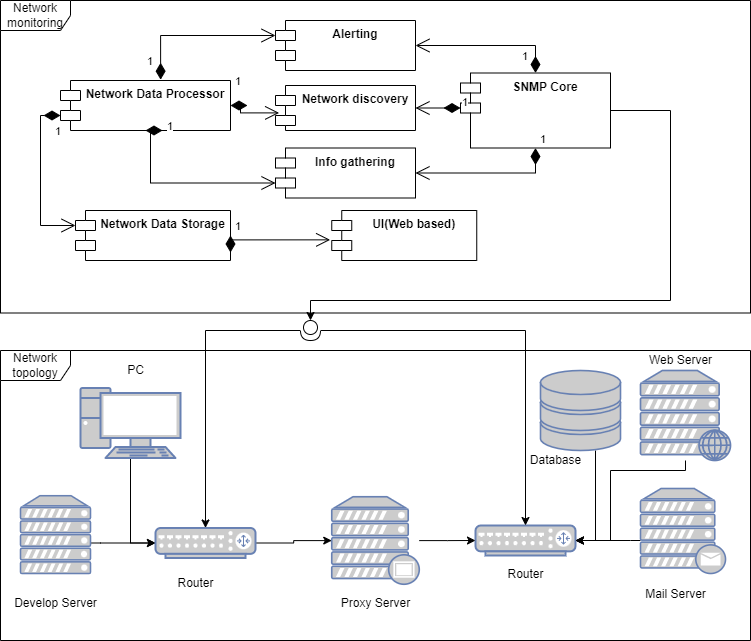
\includegraphics[scale=.55]{./diagram}
\caption{نمودار بلوکی اجزای سامانه}\label{fig.11}
\end{figure}


سپس ماژول کشف عناصر تحت مدیریت شبکه در نظر گرفته می‌شود، که به کمک ماژول هسته وظیفه جمع‌آوری اطلاعات ساختاری شبکه را بر عهده دارد. بعد از آن ماژول جمع‌آوری اطلاعات، عملکرد کل شبکه را رصد می‌کند. حال اگر زمانی با توجه به وجود اعلان‌ها نیاز به هشدار وجود داشت، از ماژول هشدار استفاده می‌شود. 

\newpage

نکته حائز اهمیت در رابطه با سه ماژول آخر این است که هر ماژول از ماژول هسته استفاده می‌کند. همچنین اطلاعاتی که هر ماژول بدست می‌آورد تحویل ماژول پردازش اطلاعات می‌دهد.

در پردازشگر اطلاعات شبکه، اطلاعات خام دریافتی از سه ماژول هشدار، کشف شبکه و جمع‌آوری اطلاعات پردازش می‌شوند تا اطلاعات قابل فهم توسط مدیر استخراج شود. حال باید اطلاعات تولید شده به ماژول ذخیره‌سازی اطلاعات داده شود.

ماژول واسط کاربری نیز در قالب یک وب سایت و فراهم آوردن یک پنل ورودی برای مدیران شبکه نیز اطلاعات ساختاری شبکه، پایش شبکه و هشدارها را از ماژول ذخیره‌سازی دریافت کرده و نمایش می‌دهد. همچنین از طریق آن می‌توان پارامترهای مختلف برای عناصر مختلف تنظیم و اقدام به اسکن کل شبکه کرد.

اما نیاز است که یک واسطی بین شبکه و سامانه مذکور باشد. در شکلی که بررسی شد، سامانه به یک شبکه فرضی از طریق مسیریاب‌های آن متصل است. در واقع واسط بین سامانه و شبکه ماژول هسته \lr{SNMP} خواهد بود.






\section{خلاصه}
% 1


هدف نهایی این فصل طراحی معماری سامانه بود. برای این امر ابتدا زیرمجموعه‌ای از ویژگی‌های سامانه‌های فصل دوم ذکر شد.

سپس با تحلیل نیازمندی‌ها دو جدول نیازمندی‌های کارکردی و غیرکارکردی تولید شد. در نهایت بعد از تولید نیازمندی‌ها به بررسی فناوری‌های پیاده‌سازی بخش‌های مختلف پرداخته شد. در نهایت نیز با توجه به فناوری‌های انتخاب شده، معماری جهت توسعه نرم‌افزار طراحی شد.


\chapter{پیاده‌سازی}

در بخش قبلی معماری کلی سامانه و ماژول‌های موردنیاز برای پیاده‌سازی سامانه پایش شبکه بیان و به صورت اجمالی معرفی شدند. این فصل به چگونگی قرار گرفتن و ارتباط بخش‌های مختلف می‌پردازد و پیاده‌سازی سیستم را توضیح خواهد داد.


ماژول‌های تعریف شده در فصل قبل برای سامانه پایش شبکه‌های کامپیوتری را می‌توان در چهار دسته کلی قرار داد: 

\begin{itemize}
    \item هسته \lr{SNMP}
    \item واسط کاربری 
    \item سمت سرور
    \item ذخیره‌سازی اطلاعات


\end{itemize}

در ادامه برای هر دسته توضیحاتی ارائه خواهد شد. این توضیحات شامل ماژول‌های دربرگیرنده آن، بررسی راه‌های ممکن برای پیاده‌سازی هر ماژول و درنهایت نحوه پیاده‌سازی آن ماژول خواهد بود. 


\section{هسته \lr{SNMP}}

این دسته فقط شامل ماژول هسته \lr{SNMP} از \cref{fig.11} است. در این ماژول، هدف توسعه ابزاری است که بتوان از طریق آن انواع پیام‌های \lr{SNMP} را ارسال و دریافت کرد. بدین منظور با تعریف دو کلاس تله\LTRfootnote{\lr{Trap}} و نشست\LTRfootnote{\lr{Session}} این ماژول را پیاده‌سازی می‌کنیم. توجه شود که کتابخانه \lr{net-snmp} به زبان \lr{C} است ولی این ماژول جهت توسعه بهینه در زبان \lr{C++} توسعه داده شد. در نهایت ابزاری برای این ماژول تولید شد که قابلیت دریافت پیام‌های تله و همچنین ارسال و دریافت پیام‌هایی از نوع  \lr{get} و \lr{walk} را دارد\cite{Mirfendereski_Centom}.

\newpage

\section{واسط کاربری}

این دسته فقط شامل ماژول واسط کاربری تحت وب از \cref{fig.11} است. این قسمت برای توسعه بهینه همانطور که در فصل قبل گفته شد با چارچوب ری‌اکت توسعه داده شد. در این قسمت قدم به قدم واسط کاربری توسعه داده شده به همراه کارایی آن مورد بررسی قرار می‌دهیم\cite{Mirfendereski_Centom}.


در \cref{fig.12} و \cref{fig.13} فهرست امکانات سامانه نشان داده می‌شود که شرح مختصری از آن‌ها در ادامه آورده شده است:


\begin{figure}[!h]
    \centering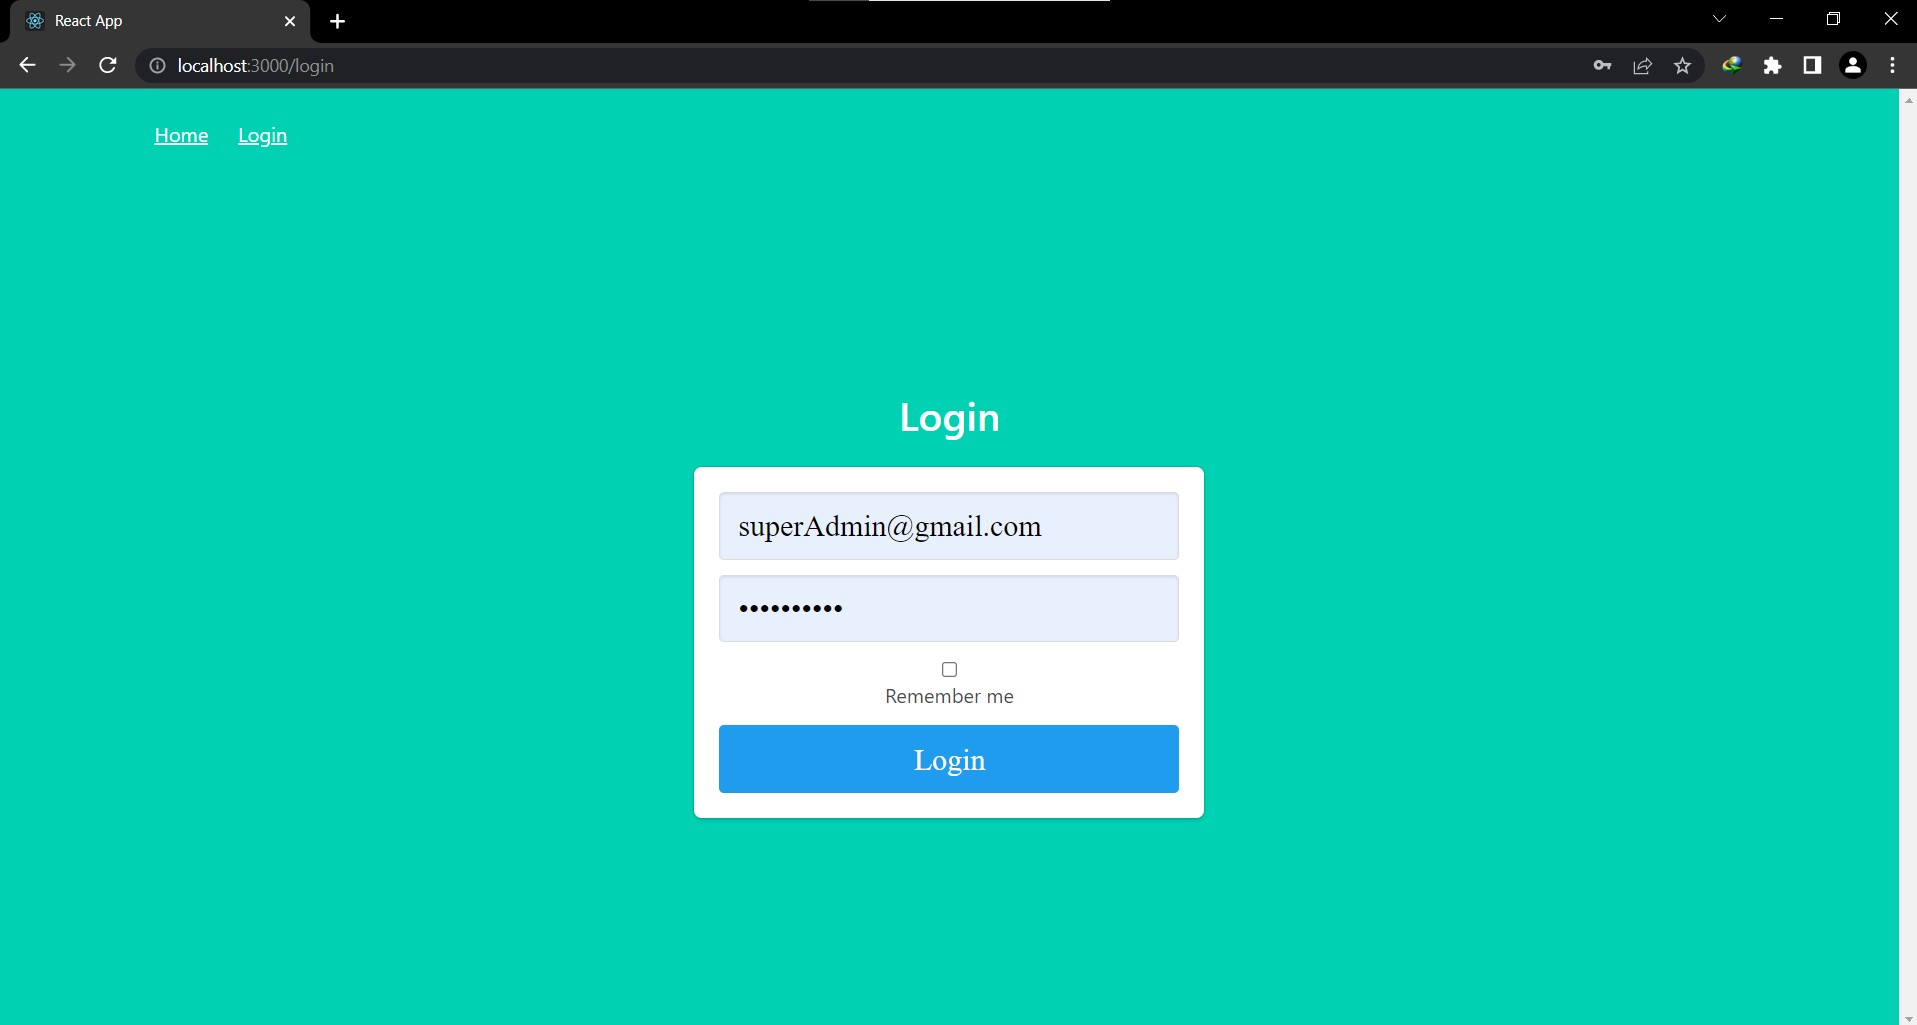
\includegraphics[scale=.38]{./nav-logout}
    \caption{فهرست امکانات سیستم هنگام ورود}\label{fig.12}
\end{figure}

\begin{figure}[!h]
    \centering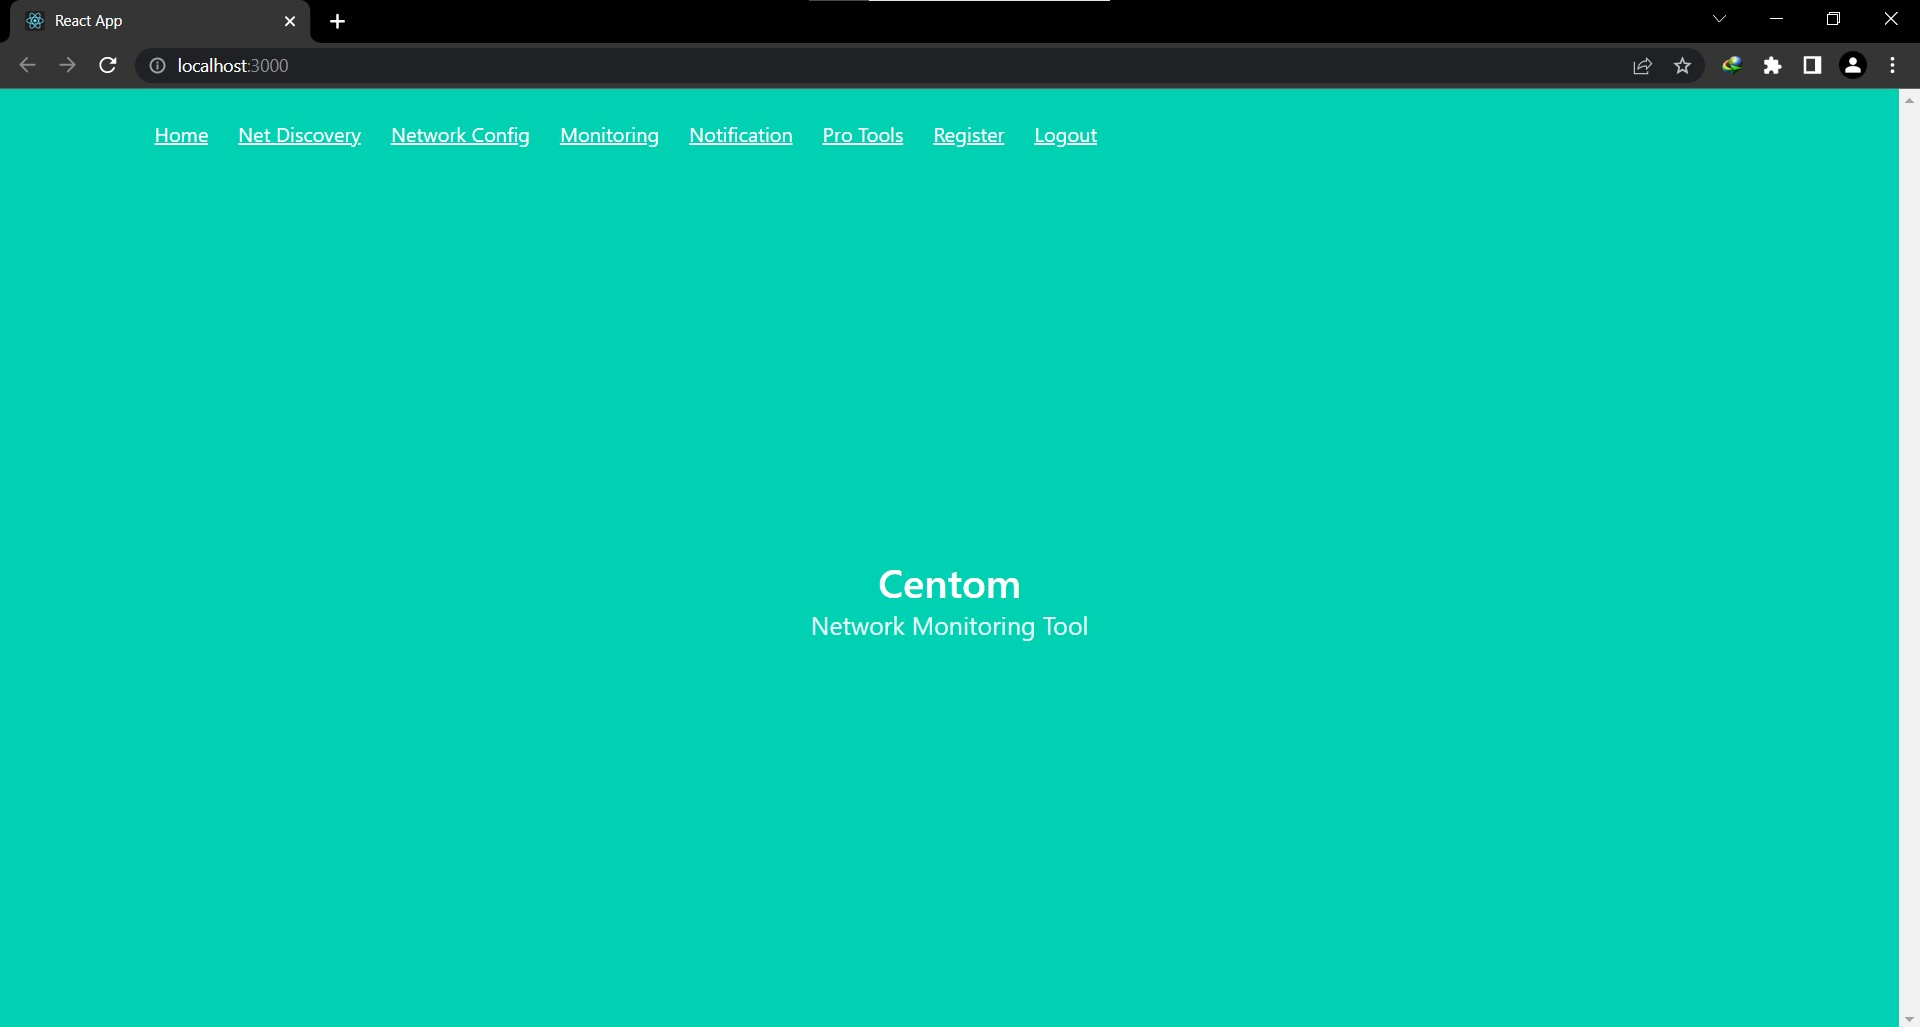
\includegraphics[scale=.38]{./nav-login}
    \caption{فهرست امکانات سیستم بعد از ورود مدیر ارشد}\label{fig.13}
\end{figure}
        
زمانی که کاربری وارد سیستم نشده است (\cref{fig.12})، تنها دو صفحه خانه و ورود به سامانه قابل دسترسی خواهد بود. این بدان علت است که در این سامانه ثبت‌نام\LTRfootnote{\lr{Register}} کاربر فقط توسط مدیر ارشد صورت می‌گیرد. در \cref{fig.13} فهرست امکانات پس از ورود مدیر ارشد نمایش داده شده‌اند. تاکیر بر روی مدیر ارشد بدین علت است که در این سامانه سه سطح دسترسی مدیر ارشد، مدیر معمولی و کاربر عادی وجود دارد. مدیر ارشد به همه امکانات دسترسی دارد. همچنین مدیر معمولی به ثبت‌نام کاربر جدید، تنظیمات و اسکن شبکه دسترسی ندارد. کاربر عادی نیز فقط به اسکن سریع یک دستگاه دسترسی خواهد داشت. البته لازم به ذکر است که سامانه یک مدیر ارشد دارد!

\newpage

تعریف کاربر جدید فقط توسط مدیر ارشد تحت صفحه ثبت‌نام در \cref{fig.14} ممکن خواهد بود. برای ثبت‌نام یک کاربر، مدیر ارشد ابتدا باید یک پست الکترونیکی\LTRfootnote{\lr{Email}} و رمز عبور وارد نماید. سپس باید برای سطح دسترسی بین دو نقش مدیر معمولی و یا کاربر معمولی انتخاب نماید. در نهایت نیز پست الکترونیکی و رمز عبور را در اختیار شخص متقاضی قرار می‌دهد.


\begin{figure}[!h]
    \centering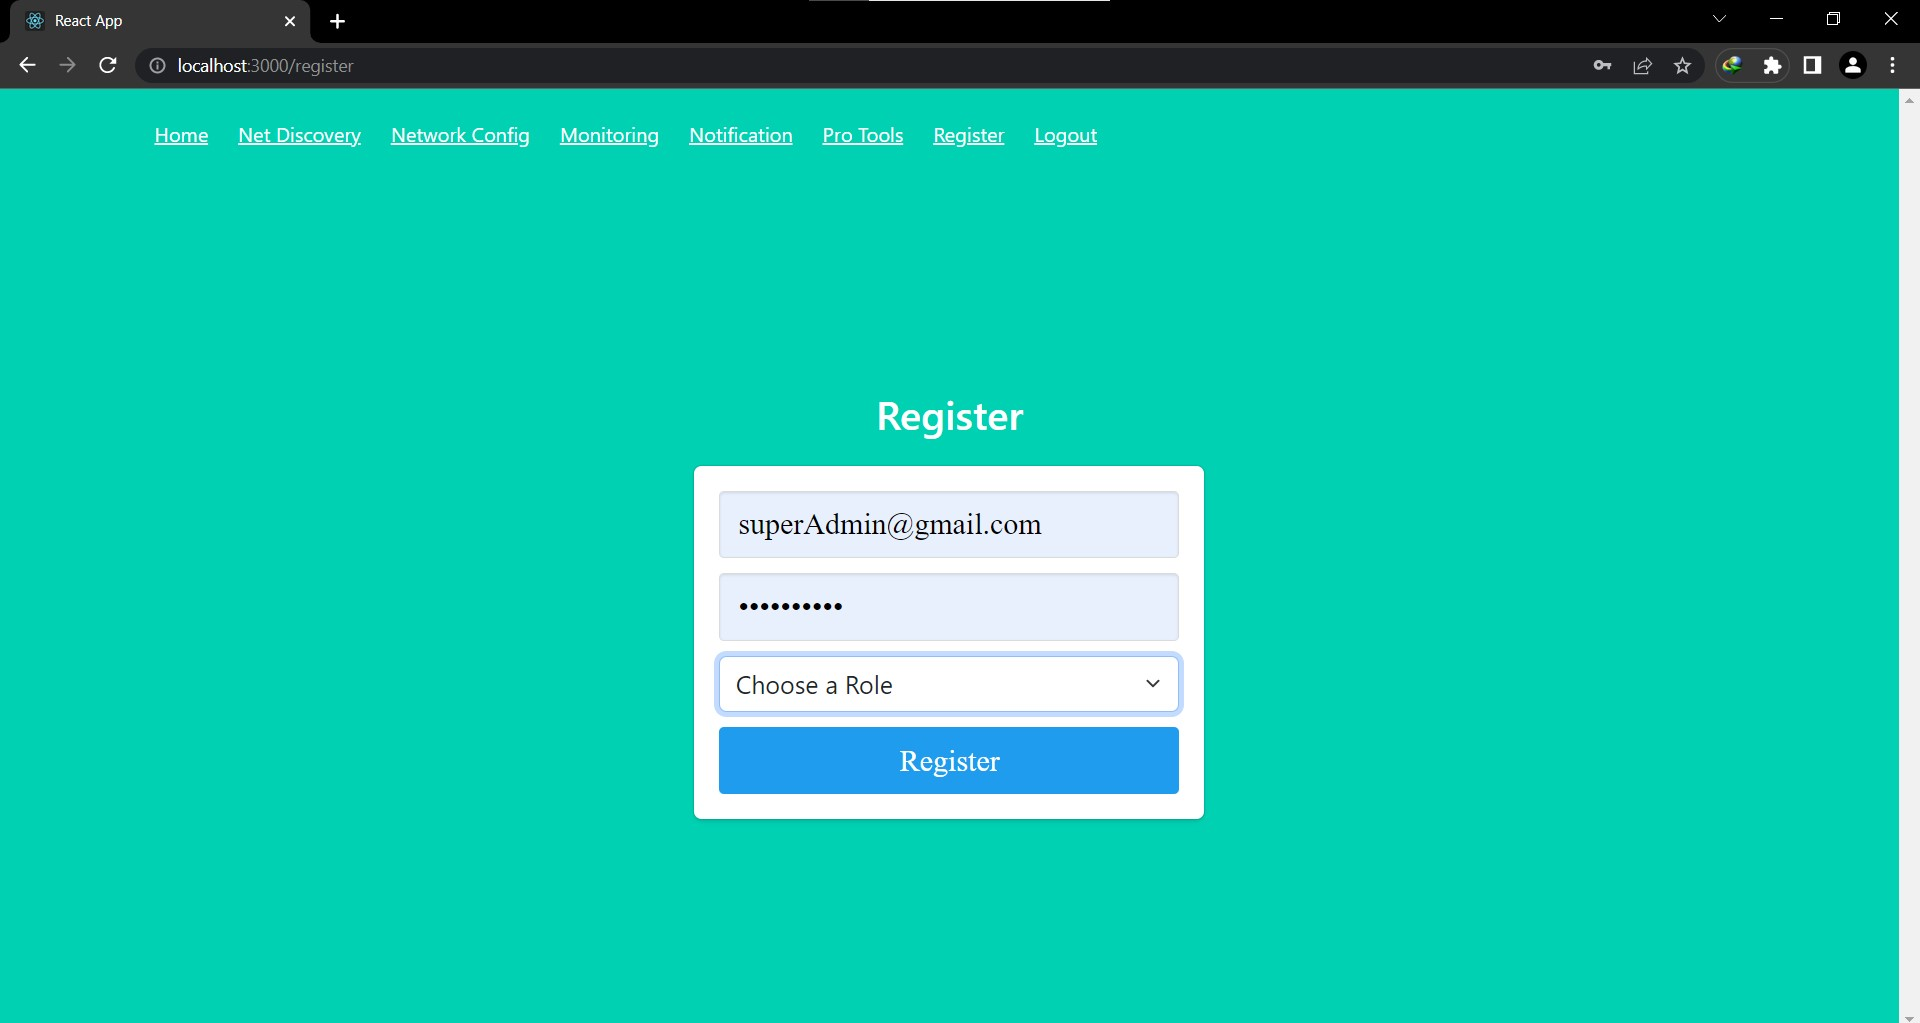
\includegraphics[scale=.35]{./register}
    \caption{صفحه ثبت‌نام در اختیار مدیر ارشد}\label{fig.14}
\end{figure}

\cleardoublepage

مهم‌ترین قسمت این سامانه، کشف شبکه است که اولین گزینه بعد از صفحه خانه قرار دارد. واسط کاربری این قسمت قبل و بعد از تست در \cref{fig.15} و \cref{fig.16} نشان داده شده‌ است. 


\begin{figure}[!h]
    \centering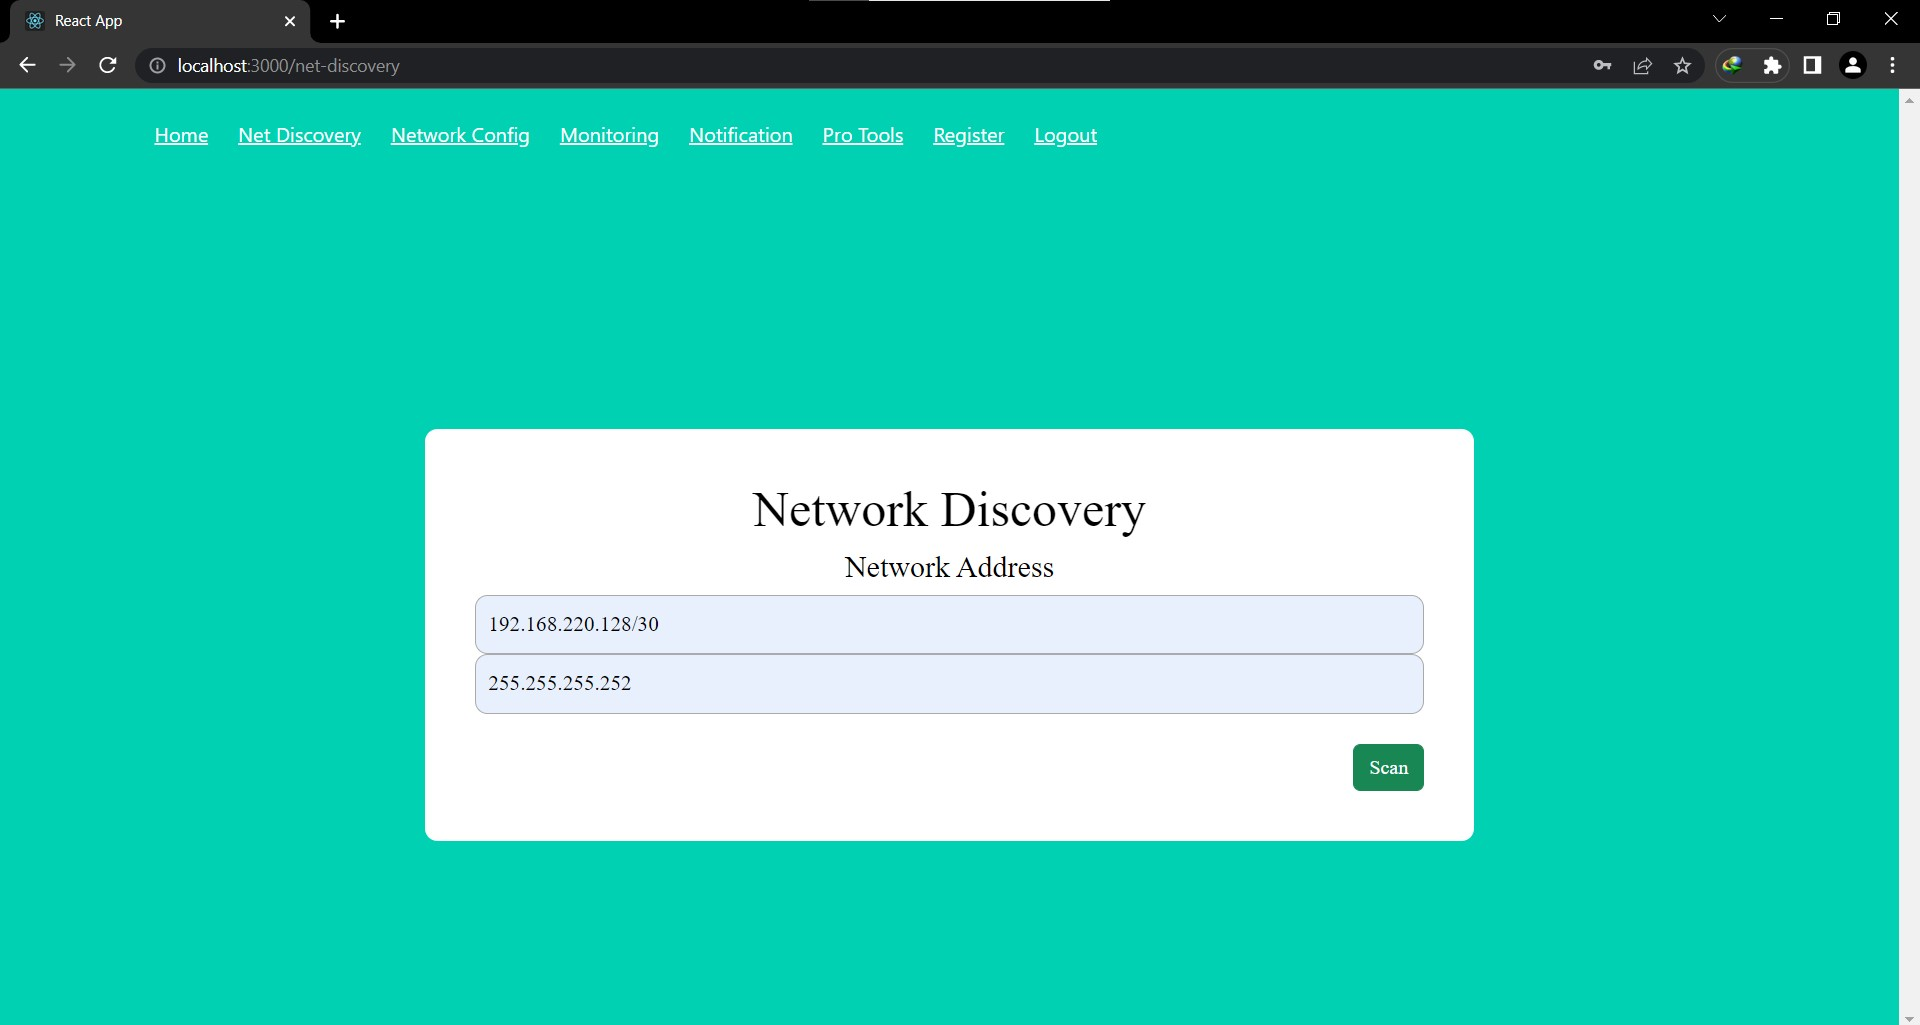
\includegraphics[scale=.38]{./net-dis-before}
    \caption{صفحه کشف شبکه قبل از اسکن}\label{fig.15}
\end{figure}


\begin{figure}[!h]
    \centering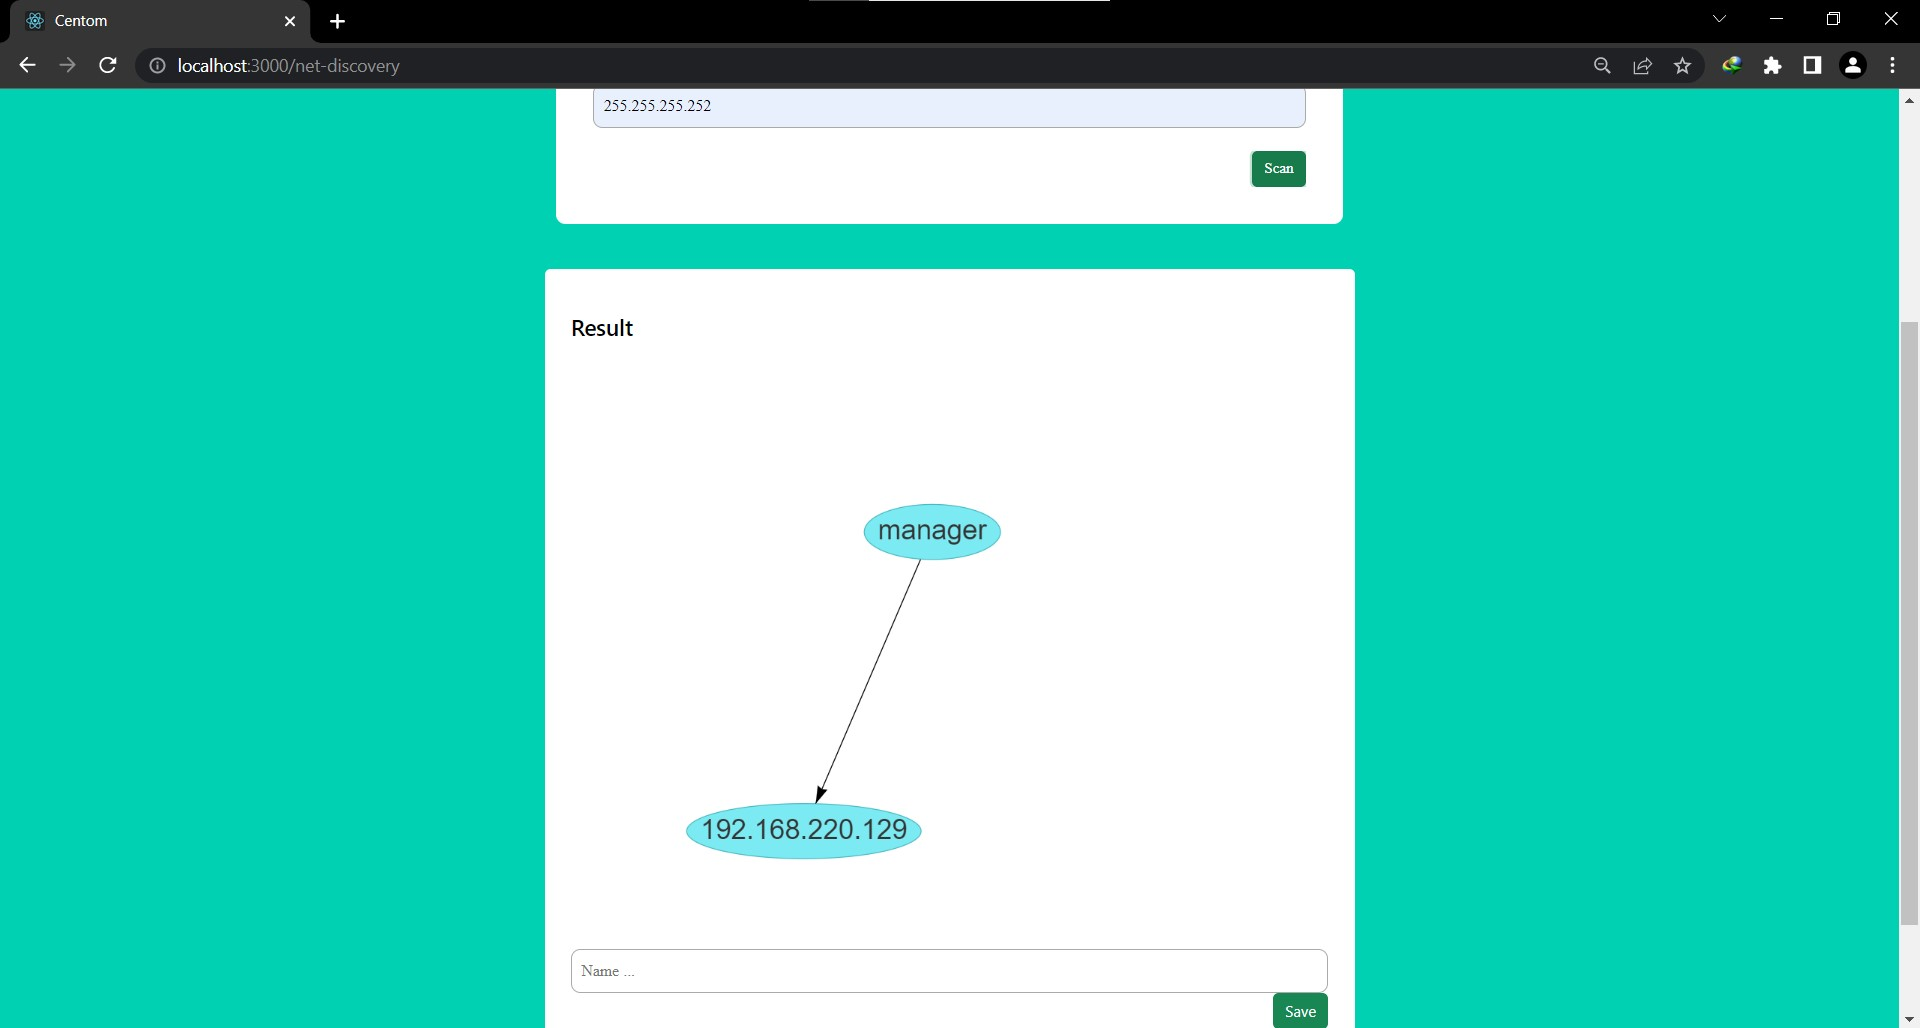
\includegraphics[scale=.38]{./net-dis-after}
    \caption{خروجی اسکن شبکه در قالب یک گراف}\label{fig.16}
\end{figure}

\cleardoublepage

در کشف شبکه ابتدا یک آدرس شبکه به همراه نقاب زیر شبکه\LTRfootnote{\lr{Subnet Mask}} از مدیر ارشد گرفته می‌شود. سپس بعد از اتمام اسکن شبکه، خروجی در قالب یک گراف نمایش داده می‌شود. درنهایت مدیر ارشد می‌تواند در صورت نیاز شبکه را با اسمی دلخواه در سامانه ذخیره کند.


بعد از ذخیره‌ سازی شبکه در قسمت قبل، مدیر ارشد می‌تواند ابتدا اطلاعات و تنظیمات شبکه را وارد نماید و بعد از آن اقدام به پایش شبکه کند. بدین ترتیب بعد از صفحه کشف شبکه، صفحه ذخیره تنظیمات شبکه در \cref{fig.17} وجود دارد. ابتدا با انتخاب اسم شبکه و نوع دستگاه‌های مورد نظر سامانه لیستی از آدرس‌ها را نشان می‌دهد. که با انتخاب یک آدرس مشخصات آن توسط کاربر وارد می‌شود. همچنین می‌تواند پارامترهای مورد نظر برای پایش دستگاه را به صورت لیست اضافه کند.



\begin{figure}[!h]
    \centering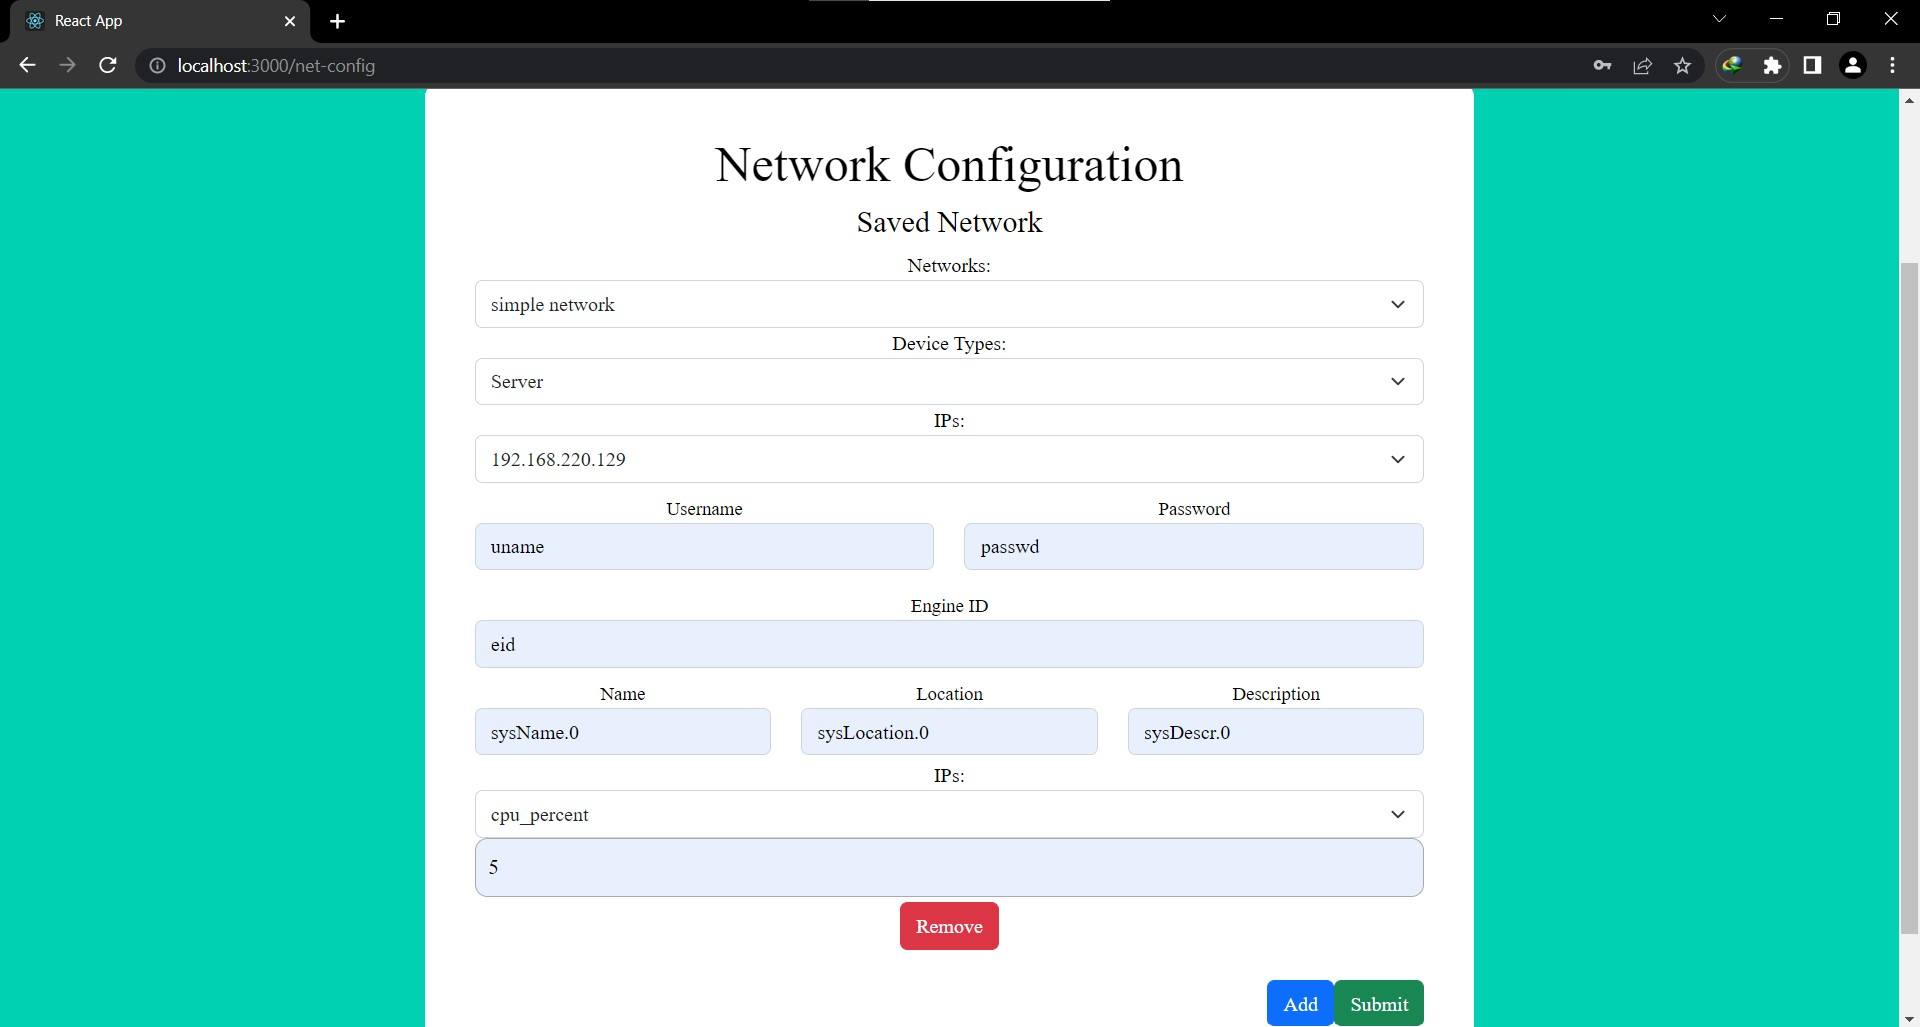
\includegraphics[scale=.38]{./net-config}
    \caption{صفحه ذخیره تنظیمات شبکه}\label{fig.17}
\end{figure}


% مانیتورینگ ///////////////////////////////////////////////////////////////////////////////////////////////////////
بعد از دریافت تنظیمات شبکه در مرحله قبل حال نوبت به پایش شبکه مورد نظر می‌رسد. این امر در صفحه پایش شبکه طبق \cref{fig.18} محقق می‌‎شود. در این صفحه بعد از انتخاب شبکه دلخواه و یک \lr{IP} مشخص، سامانه اقدام به پایش عملکرد دستگاه مورد نظر خواهد کرد.


\begin{figure}[!h]
    \centering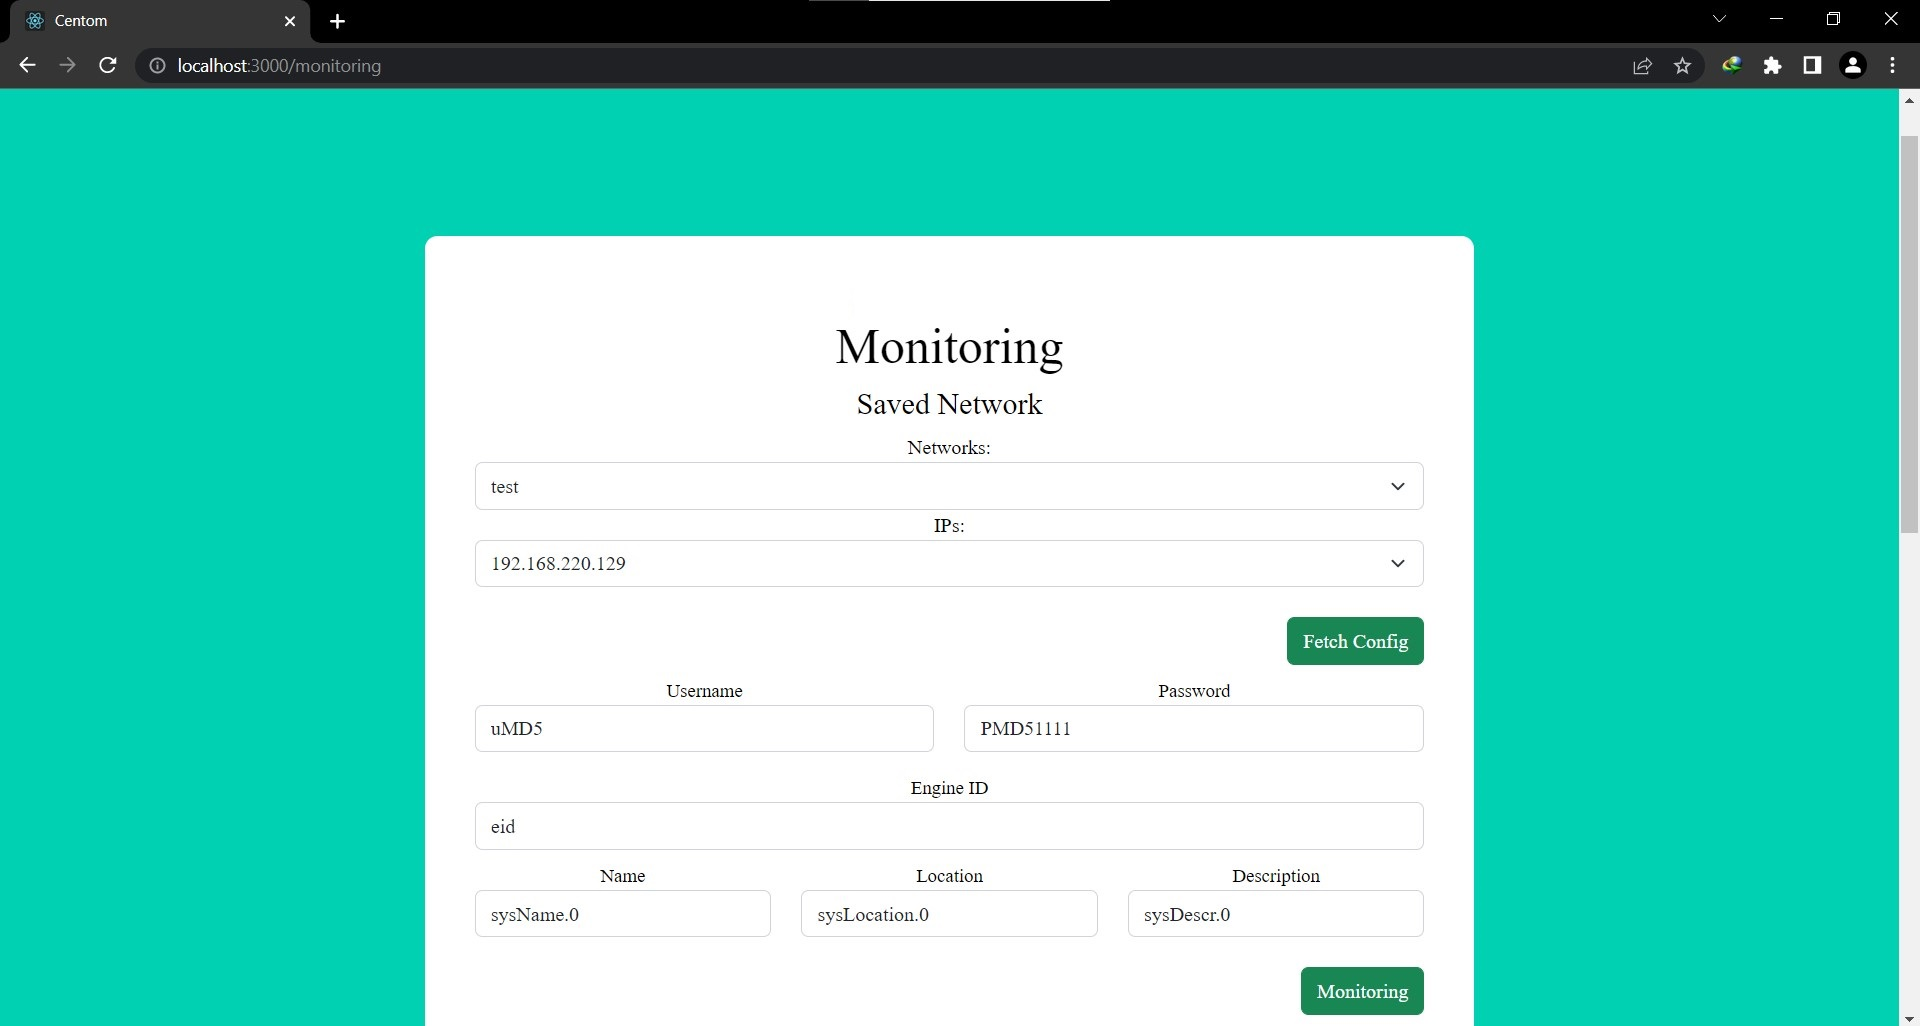
\includegraphics[scale=.38]{./monitoring}
    \caption{صفحه پایش شبکه}\label{fig.18}
\end{figure}


% نوتیفیکیشن //////////////////////////////////////////////////////////////////////////////////////////////////////

بعد از گزینه صفحه پایش، طبق معماری سامانه، صفحه اعلانات طبق \cref{fig.19} قرار دارد. در این صفحه پس از فشردن دکمه مورد نظر، سامانه به پورت 162 گوش می‌دهد و تله‌های دریافتی را در قالبی خوانا به مدیر نمایش می‌دهد.

\begin{figure}[!h]
    \centering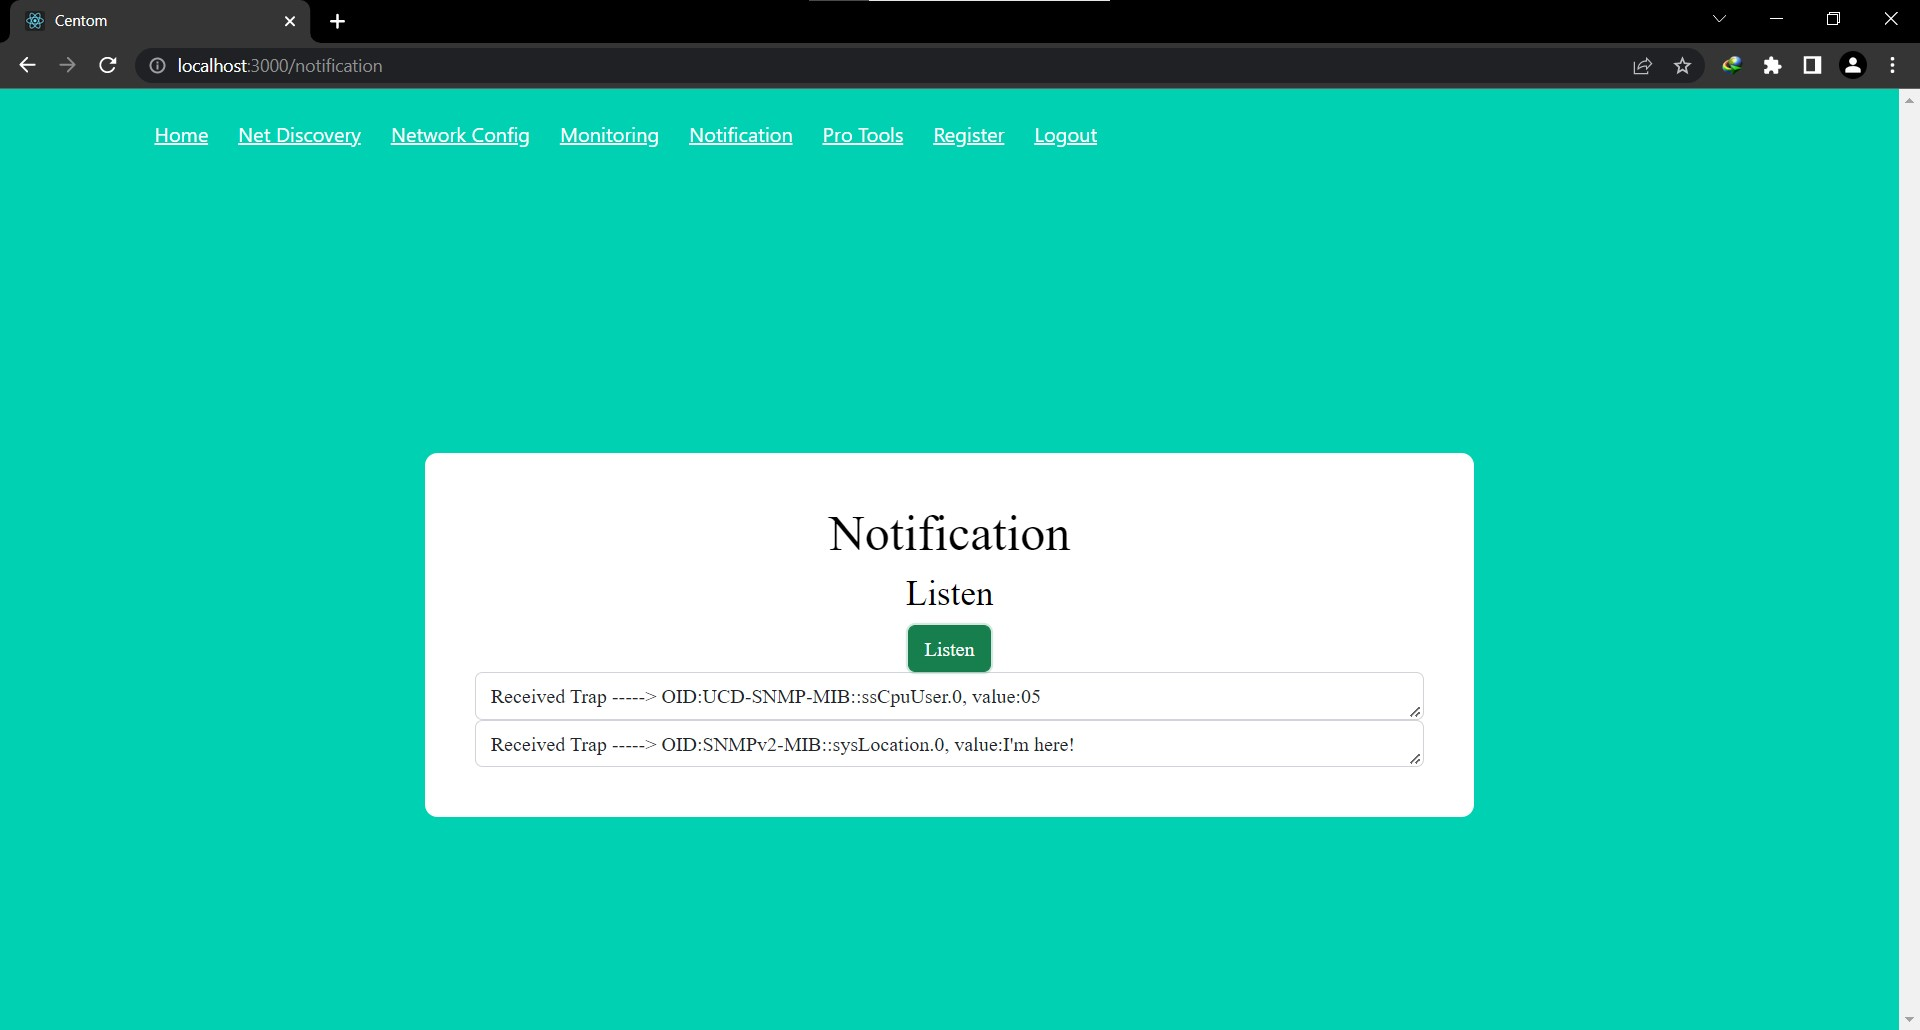
\includegraphics[scale=.38]{./notification}
    \caption{صفحه اعلانات دریافتی از شبکه}\label{fig.19}
\end{figure}

\cleardoublepage

در نهایت صفحه ابزارهای پیشرفته قرار دارد، که در حال حاضر تنها اسکن سریع آن در \cref{fig.120} موجود است. سامانه در این قسمت می‌تواند با دریافت یک آدرس و یک شناسه شی\LTRfootnote{\lr{Object Identifiers}}، پیام‌های \lr{get} و \lr{walk} را ارسال و نتیجه را به ترتیب مشاهده کند. 

\begin{figure}[!h]
    \centering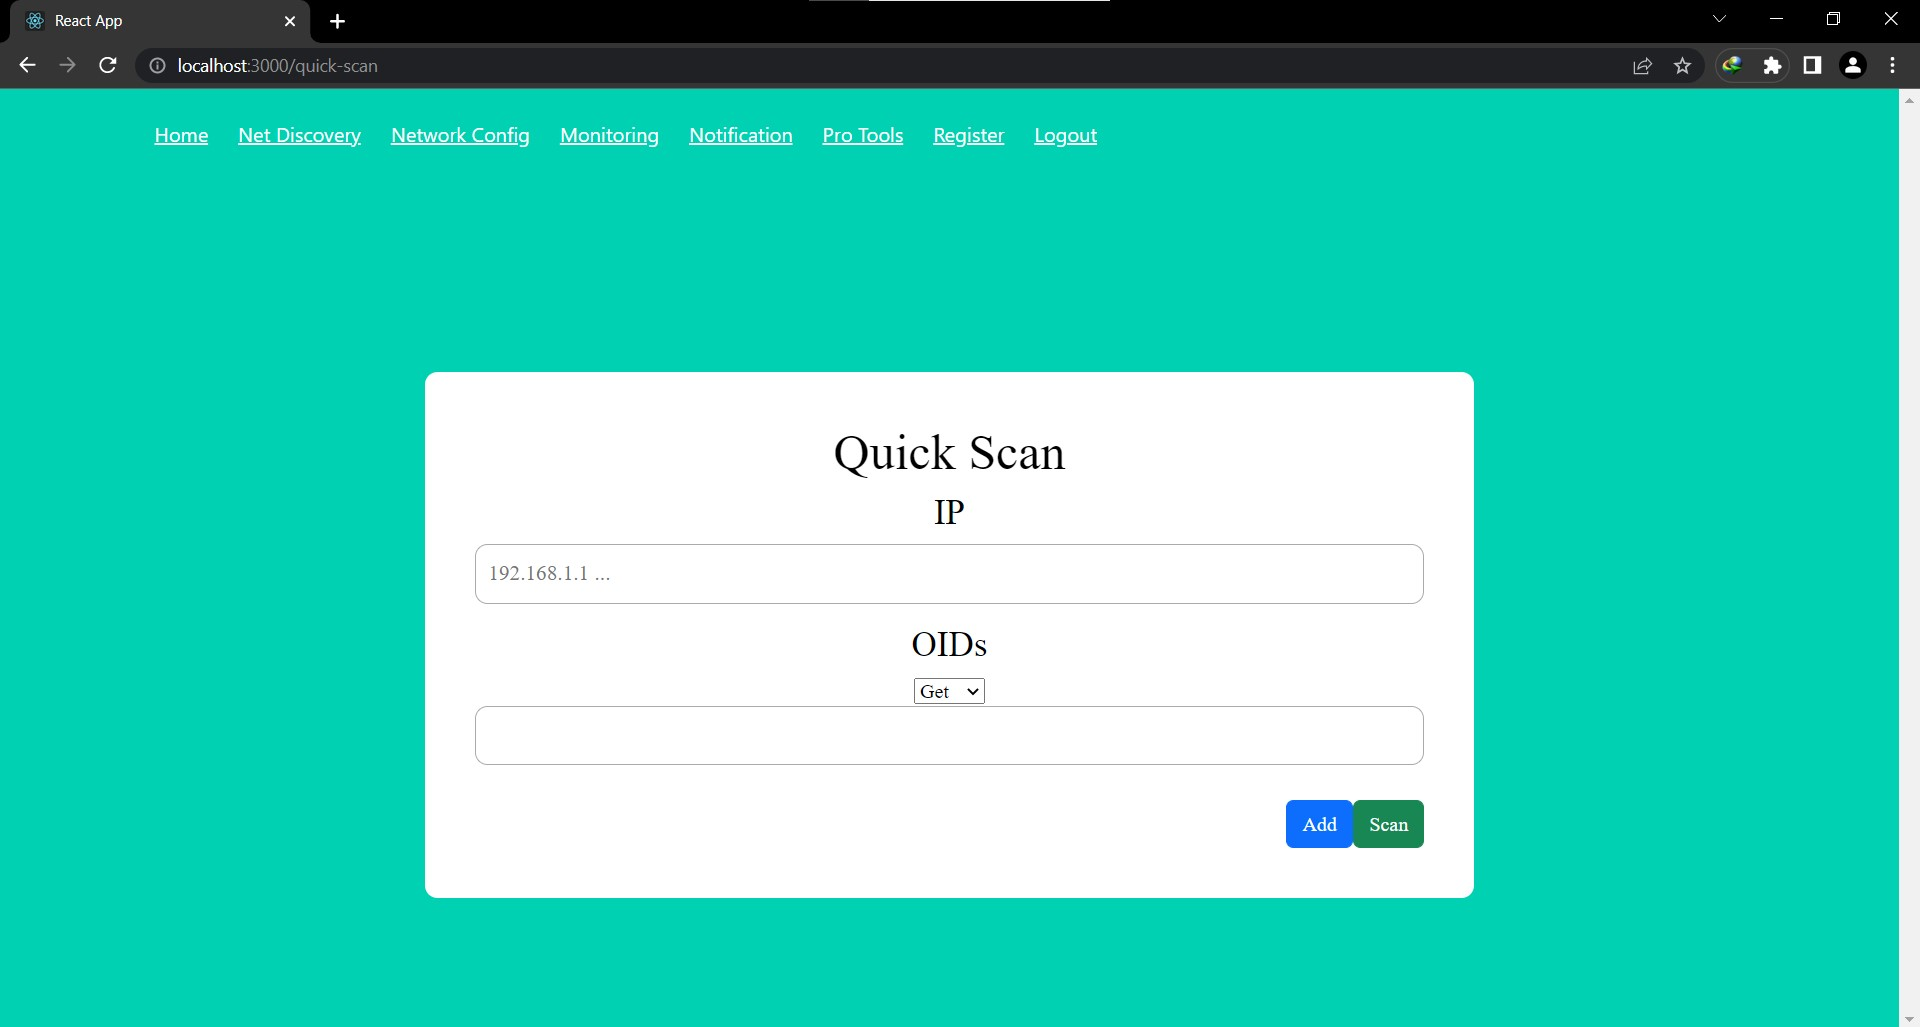
\includegraphics[scale=.38]{./pro-tools}
    \caption{صفحه ابزارهای پیشرفته}\label{fig.120}
\end{figure}



\cleardoublepage

\section{ذخیره‌سازی اطلاعات}

این دسته فقط شامل ماژول ذخیره‌سازی اطلاعات شبکه از \cref{fig.11} است. در این سامانه به طور کلی سه نوع داده کاربران، اطلاعات شبکه و اطلاعات دریافتی از عناصر تحت مدیریت شبکه وجود دارد\cite{Mirfendereski_Centom}.



\subsection{ذخیره‌سازی اطلاعات شبکه و کاربران}

برای ذخیره‌سازی اطلاعات کاربران و اطلاعات شبکه از پایگاه داده \lr{SQLite} با تعریف جدول‌ها شکل \cref{fig.121} استفاده می‌کنیم.

\begin{figure}[!h]
    \centering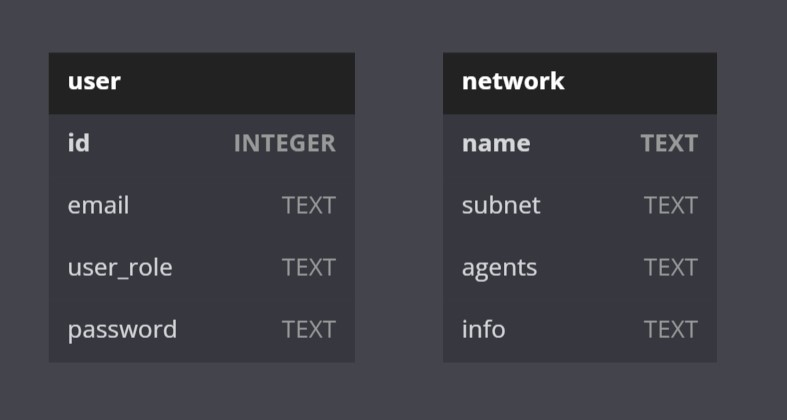
\includegraphics[scale=.60]{./db}
    \caption{تصویر جدول‌های تعریف شده در پایگاه داده \lr{SQLite}}\label{fig.121}
\end{figure}


فیلدهایی که نیاز است توضیحی درباره آن‌ها داده شود به صورت زیر است:

\begin{itemize}
    \item \lr{user-role}: نقش هر کاربر جهت دسترسی ‌های متنوع به سامانه را می‌دهد. به عنوان مثال مدیر ارشد به همه امکانات، مدیر معمولی به همه امکانات به جز ثبت‌نام کاربر جدید، تنظیمات و اسکن شبکه دسترسی دارند. و در نهایت کاربر عادی فقط به اسکن سریع یک دستگاه دسترسی خواهد داشت.
    \item \lr{name}: این فیلد فقط برای شناسایی متمایز شبکه‌ها کاربرد دارد. بدین صورت که با دریافت یک اسم از کاربر به هنگام ذخیره، تنها زمان بازیابی اطلاعات شبکه در سامانه کاربرد دارد.
    \item \lr{agents}: این فیلد شامل لیستی از دستگاه‌های شبکه است که عامل \lr{SNMP} بر روی آن‌ها فعال است.
    \item \lr{info}: این فیلد شامل شی‌ای از \lr{JSON}\LTRfootnote{\lr{JavaScript Object Notation}} شامل گره‌ها، یال‌ها و نوع دستگاه‌های تحت مدیریت است.

\end{itemize}


برای اتصال به پایگاه داده \lr{SQLite} نیز از \lr{SQLAlchemy} که یک ابزار نگاشت رابطه به شی\LTRfootnote{\lr{Object–relational mapping (ORM)}} است، استفاده شد که مزایای بسیاری دارد.



\subsection{ذخیره‌سازی اطلاعات دریافتی از شبکه}

این اطلاعات در درجه اول شامل پارامتر‌های مختلف جهت پایش دستگاه‌ها به همراه نرخ نمونه‌برداری\LTRfootnote{\lr{rate}} آن‌ها است. در درجه بعد شامل اطلاعات دریافتی از دستگاه‌های تحت مدیریت مربوط به پارامترهای مختلف خواهد بود. به علت تعداد بالای بازیابی این گونه اطلاعات از ردیس استفاده شد. برای اتصال به ردیس نیز از ماژول ردیس در پایتون استفاده شد.

\newpage

\section{سمت سرور}

این دسته شامل ماژول‌های پردازش اطلاعات شبکه، هشدار، کشف شبکه و جمع‌آوری اطلاعات (پایش) از \cref{fig.11} است. ادامه این فصل به بررسی ماژول‌های گفته شده می‌پردازد.


\subsection{ماژول کشف شبکه}

در این ماژول با توجه به نیازمندی‌های گفته شده در فصل تحلیل و طراحی، سامانه باید قادر باشد تا با دریافت یک آدرس شبکه، عناصری که عامل \lr{SNMP} بر روی آن‌ها فعال هستند را به همراه نوع عنصر (سرور، مسیریاب، سوییچ و تکرارکننده) آن‌ها مشخص کند. این خروجی باید بر اساس یک توپولوژی شبکه باشد.


این مسئله با توسعه یک الگوریتم مشخص باید حل شود. در ادامه تکنیک‌های موجود برای حل این مسئله بیان و بررسی می‌شوند. در نهایت نیز راه حل به کار گرفته شده ارائه می‌شود.

تکنیک‌های حل این مسئله:

\begin{itemize}
    \item استفاده از پینگ\LTRfootnote{\lr{Ping}} همه پخشی\LTRfootnote{\lr{Broadcast}} برای شناسایی تمام عناصر شبکه
    \item استفاده از پروتکل‌های کشف لایه پیوند\LTRfootnote{\lr{Link Layer Discovery Protocol (LLDP)}} و یا کشف سیسکو\LTRfootnote{\lr{Cisco Discovery Protocol (CDP)}}
    \item استفاده از پیام \lr{SNMP} با شناسه شی \lr{sysServices.0}
\end{itemize}

به علت عدم پشتیبانی بعضی از دستگاه‌ها از پروتکل‌های کشف لایه پیوند و کشف سیسکو و یا نیاز به ابزارهایی اضافی جهت حل این مسئله، از این دو پروتکل استفاده نشد. اما الگوریتمی که برای این مسئله توسعه داده شد به شرح زیر می‌باشد\cite{Mirfendereski_Centom}:

\begin{enumerate}
    \item ارسال یک پیام \lr{SNMP} با شناسه شی \lr{ sysServices.0} به تمام آدرس‌های موجود در آدرس شبکه (اگر پاسخی دریافت شود یعنی عنصر نیازمند مدیریت است.)
    \item رمز گشایی مقدار مرحله قبل در صورت دریافت پاسخ از آدرس مربوطه به صورت زیر:
    \begin{enumerate}
        \item تبدیل عدد برگردانده شده به فرمت باینری و تعیین نوع عنصر بر اساس مقادیر بیت‌ها (کم ارزش ترین بیت، بیت اول در نظر گرفته می‌شود)
        \item اگر بیت اول تنظیم شده باشد، دستگاه موردنظر یک نوع تکرارکننده است.
        \item اگر بیت دوم تنظیم شده باشد، دستگاه موردنظر یک نوع سوییچ است.
        \item اگر بیت سوم تنظیم شده باشد و همچنین مقدار پیام \lr{SNMP} با شناسه شی \lr{ ipForwarding.0 } یک باشد، دستگاه موردنظر یک نوع مسیریاب است.
        \item اگر هیچ کدام از موارد بالا نباشد و همچنین بیت چهارم یا هفتم تنظیم شده باشد، دستگاه موردنظر یک نوع سرور است.
        \item اگر مقدار برگردانده شده در موارد بالا صدق نمی‌کرد، نوع دستگاه متفرقه\LTRfootnote{\lr{Other}} خواهد بود (مثل یک دستگاه منبع تغذیه اضطراری\LTRfootnote{\lr{Uninterruptible Power Supply (UPS)}}). 
    \end{enumerate}
    \item به ازای تمام آدرس‌هایی که عامل \lr{SNMP} بر روی آن‌ها در حال اجرا هستند، دستور \lr{traceroute} اجرا می‌شوند. خروجی بدین صورت خواهد بود که تا رسیدن به مقصد نهایی گام‌های میانی نمایش داده می‌شوند. بدین ترتیب به تعداد عناصر فعال، مسیرهای رسیدن تا آن‌ها بدست می‌آیند.
    \item در نهایت برای رسم توپولوژی شبکه تحت یک گراف، با داشتن گره‌ها و همچنین یال‌های بدست آمده از مسیرها این امر ممکن می‌شود.
\end{enumerate}




\subsection{ماژول پردازش اطلاعات شبکه}

در این ماژول اطلاعات دریافت شده از سمت دستگاه‌های شبکه یعنی همان پیام‌های \lr{SNMP}، با توجه به مقدار آن‌ها پردازش می‌شوند. این پردازش شامل دو قسمت یعنی ابتدا نوع داده دریافتی را مشخص کرده و بعد از در صورت نیاز به حذف تعدادی کاراکتر از آن، اقدام می‌شود. قسمت دوم این پردازش بدین جهت خواهد بود که به عنوان مثال بعضی مقادیر حجم حافظه و ... در انتها عبارت \lr{KB} وجود دارد.

\subsection{ماژول جمع‌آوری اطلاعات }

برای راحتی انجام پایش و تنظیمات شبکه توسط سامانه، در پروژه یک فایل با پسوند \lr{JSON} طبق \cref{fig.122} تعبیه شده است. در این فایل دو نوع کلید وجود دارد. اولین کلید، پارامترهای پیش‌فرض\LTRfootnote{\lr{def\_params}} است. اهمیت بعضی پارامترها باعث اضافه شدن این بخش شد تا این پارامترها برای تمام دستگاه‌ها بدون نیاز به افزودن توسط مدیر ارشد رصد شوند. در ادامه هر کلید متعلق به این کلید، برای یک پارامتر به خصوص شامل شناسه شی، نرخ نمونه‌برداری و نحوه پردازش آن برای نمایش است. ساختار زیرین دومین کلید یعنی پارامترها\LTRfootnote{\lr{params}} نیز به همین صورت است. با این تفاوت که به مدیر ارشد لیستی از این موارد نشان داده شده و او می‌تواند برای هر \lr{IP} در بخش تنظیمات شبکه از این لیست انتخاب نماید. در ادامه نیز برای ارسال اطلاعات به صورت بی‌درنگ\LTRfootnote{\lr{real-time}} از \lr{SSE}\LTRfootnote{\lr{Server-Sent Events}} استفاده شد. که توسعه آن در فلسک و ری‌اکت کمی با چالش نیز همراه بود\cite{Mirfendereski_Centom}.


\begin{figure}[!h]
    \centering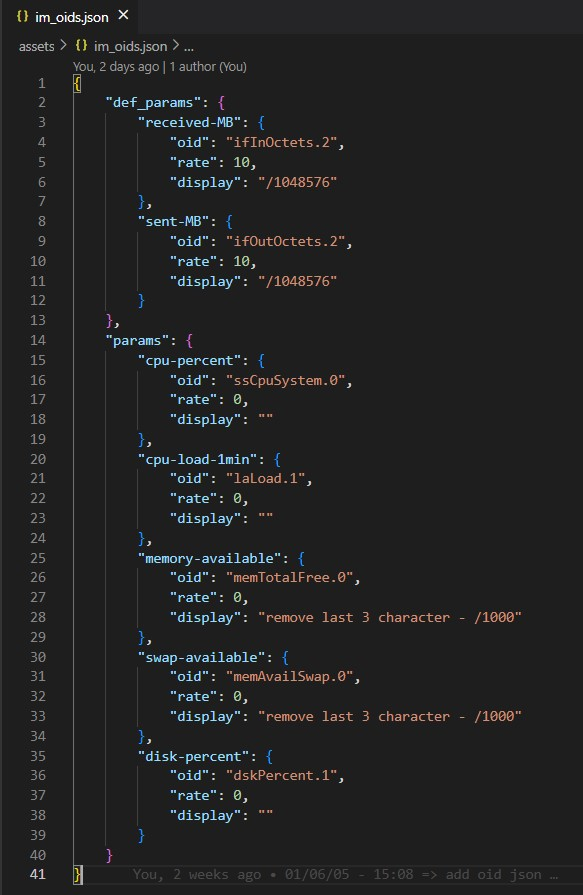
\includegraphics[scale=.80]{./im-json}
    \caption{تصویر فایل \lr{JSON} جهت مدیریت پارامترها}\label{fig.122}
\end{figure}




\subsection{ماژول هشدار}

ماژول هشدار که در قالب کلاس تله وظیفه خود را انجام می‌دهد. این ماژول باید دریافت اطلاعات و تفسیر آن‌ها کار خود را انجام دهد. همچنین اشاره به این نکته که تمام پیام‌های \lr{SNMP} با \lr{asn.1}\LTRfootnote{\lr{Abstract Syntax Notation One}} کدگذاری\LTRfootnote{\lr{encode}} و ارسال می‌شوند، لازم است. در واقع کاری که کلاس تله انجام می‌دهد را می‌توان به صورت مراحل زیر بیان کرد\cite{Mirfendereski_Centom}:

\begin{enumerate}
    \item گوش دادن به پورت 162 و دریافت اطلاعات
    \item تبدیل اطلاعات در قالب هگزادسیمال\LTRfootnote{\lr{hexadecimal}} به فرمت رشته\LTRfootnote{\lr{String}} در زبان \lr{C++}
    \item حذف کاراکترهای فاصله در رشته
    \item کدگشایی\LTRfootnote{\lr{decode}} رشته مورد نظر با \lr{asn.1} از طریق ابزارهای \lr{xxd} و \lr{openssl}

\end{enumerate}


\section{خلاصه}

این فصل با توجه به معماری طراحی شده در فصل قبل، با گروه‌بندی ماژول‌ها، نحوه پیاده‌سازی هر ماژول بیان شد. در ابتدا نحوه پیاده‌سازی هسته \lr{SNMP} بیان شد. بعد از آن به توضیح پیاده‌سازی واسط کاربری پرداخته شد. در ادامه نیز ذخیره‌سازی اطلاعات و درنهایت سمت سرور توضیح داده شدند. بخش سمت سرور نیز خود از چندین ماژول پردازش اطلاعات شبکه، هشدار، کشف شبکه و جمع‌آوری اطلاعات (پایش) تقسیم شده و به هرکدام به تفکیک پرداخته شد.
\chapter{تست و ارزیابی سامانه}
%%%%%%%%%%%%%%%%%%%%%%%%%%%%%%%%%%%%%%%%%%%
مقدمه فصل
\chapter{امکانات لازم }

منابع و امکاناتی که ما نیاز داریم تا این سامانه را پیاده سازی کنیم به شرح زیر می‌باشد:

\begin{itemize}
    \item اینترنت
    \item سیستم شخصی جهت توسعه نرم افزار
    \item تعدادی کتابخانه‌ی عمومی که در دسترس هستند
\end{itemize}

%--------------------------------------------------------------------------appendix( مراجع و پیوست ها)
\chapterfont{\vspace*{-2em}\centering\LARGE}%

\appendix
\bibliographystyle{unsrt-fa}
\bibliography{references}
% \chapter*{‌پیوست}
\markboth{پیوست}{}
\addcontentsline{toc}{chapter}{پیوست}
موضوعات مرتبط با متن گزارش پایان نامه كه در يكی از گروه‌های زير قرار می‌گيرد، در بخش پيوست‌ها آورده شوند:
\begin{enumerate}
\item  اثبات های رياضی يا عمليات رياضی طولانی‌.‌
\item داده و اطلاعات نمونه (های) مورد مطالعه (\lr{Case Study}) چنانچه طولانی باشد‌.‌
\item نتايج كارهای ديگران چنانچه نياز به تفصيل باشد‌.‌
\item مجموعه تعاريف متغيرها و پارامترها، چنانچه طولانی بوده و در متن به انجام نرسيده باشد‌.‌
\end{enumerate}
% براي شماره‌گذاري روابط، جداول و اشكال موجود در پيوست‌ از ساختار متفاوتي نسبت به متن اصلي استفاده مي‌شود كه در زير به‌عنوان نمونه نمايش داده شده‌است. 
% \begin{equation}
%F=ma
%\end{equation}
\section*{کد میپل }
\begin{latin}
\begin{verbatim}

with(DifferentialGeometry):
with(Tensor):
DGsetup([x, y, z], M)
																	frame name: M
a := evalDG(D_x)
																	D_x
b := evalDG(-2 y z D_x+2 x D_y/z^3-D_z/z^2)


\end{verbatim}
\end{latin}
%--------------------------------------------------------------------------dictionary(واژه نامه ها)
%اگر مایل به داشتن صفحه واژه‌نامه نیستید، خط زیر را غیر فعال کنید.
\parindent=0pt
%
\chapter*{واژه‌نامه‌ی فارسی به انگلیسی}
\pagestyle{style9}

\addcontentsline{toc}{chapter}{واژه‌نامه‌ی فارسی به انگلیسی}
%%%%%%
\begin{multicols*}{2}

{\bf آ}
\vspace*{3mm}


\farsiTOenglish{اسکالر}{Scalar}


\vspace*{3mm}
{\bf ب}
\vspace*{3mm}

\farsiTOenglish{بالابر}{Lift}


\vspace*{3mm}
{\bf پ}
%%\vspace*{3mm}

\farsiTOenglish{پایا}{Invariant}



\vspace*{3mm}
{\bf ت}
%%\vspace*{3mm}

\farsiTOenglish{ تناظر }{Correspondence}


\vspace*{3mm}
{\bf ث}
%%\vspace*{3mm}

\farsiTOenglish{ثابت‌ساز}{Stabilizer}

\vspace*{3mm}
{\bf ج}
%%\vspace*{3mm}

\farsiTOenglish{جایگشت}{Permutation}



\vspace*{3mm}
{\bf چ}
%%\vspace*{3mm}


\farsiTOenglish{چند جمله‌ای }{Polynomial}

\vspace*{3mm}
{\bf ح}
%%\vspace*{3mm}

\farsiTOenglish{حاصل‌ضرب دکارتی}{Cartesian product}


\vspace*{3mm}
{\bf خ}
%%\vspace*{3mm}

\farsiTOenglish{خودریختی}{Automorphism}

\vspace*{3mm}
{\bf د}
%%\vspace*{3mm}

\farsiTOenglish{درجه}{Degree}


\vspace*{3mm}
{\bf ر}
%%\vspace*{3mm}


\farsiTOenglish{ریزپردازنده}{microprocessor}


\vspace*{3mm}
{\bf ز}
%%\vspace*{3mm}


\farsiTOenglish{زیرمدول}{Submodule}


\vspace*{3mm}
{\bf س}
%%\vspace*{3mm}

\farsiTOenglish{سرشت}{Character}


\vspace*{3mm}
{\bf ص}
%%\vspace*{3mm}

\farsiTOenglish{صادقانه}{Faithful}

\vspace*{3mm}
{\bf ض}
%%\vspace*{3mm}

\farsiTOenglish{ضرب داخلی}{Inner product}

\vspace*{3mm}
{\bf ط}
%%\vspace*{3mm}


\farsiTOenglish{طوقه}{Loop}


\vspace*{3mm}
{\bf ظ}
%%\vspace*{3mm}


\farsiTOenglish{ظرفیت}{Valency}
 
\vspace*{3mm}
{\bf ع}
%%\vspace*{3mm}


\farsiTOenglish{عدم مجاورت}{Nonadjacency}



\vspace*{3mm}
{\bf ف}
%%\vspace*{3mm}

\farsiTOenglish{فضای برداری}{Vector space}



\vspace*{3mm}
{\bf ک}
%%\vspace*{3mm}

\farsiTOenglish{کاملاً تحویل‌پذیر}{Complete reducibility}


\vspace*{3mm}
{\bf گ}
%%\vspace*{3mm}


\farsiTOenglish{گراف}{Graph}



\vspace*{3mm}
{\bf م}
%%\vspace*{3mm}

\farsiTOenglish{ماتریس جایگشتی}{Permutation matrix }


\vspace*{3mm}
{\bf ن}
%%\vspace*{3mm}

\farsiTOenglish{ناهمبند}{Disconnected}


\vspace*{3mm}
{\bf و}
%%\vspace*{3mm}

\farsiTOenglish{وارون‌پذیر}{Invertible}


\vspace*{3mm}
{\bf ه}
%%\vspace*{3mm}

\farsiTOenglish{همبند}{Connected}



\vspace*{3mm}
{\bf ی}
%%\vspace*{3mm}

\farsiTOenglish{یال}{Edge}




\end{multicols*}%
%%%%%%
\chapter*{ واژه‌نامه‌ی انگلیسی به فارسی}
\pagestyle{style9}
\lhead{\thepage}\rhead{واژه‌نامه‌ی انگلیسی به فارسی}
\addcontentsline{toc}{chapter}{واژه‌نامه‌ی انگلیسی به فارسی}

\LTRmulticolcolumns
\begin{multicols}{2}
{\hfill\bf  \lr{A}}
%%\vspace*{1.5mm}

\englishTOfarsi{Automorphism}{خودریختی}

\vspace*{3mm}
{\hfill\bf   \lr{B}}
%%\vspace*{1.5mm}

\englishTOfarsi{Bijection}{دوسویی}

\vspace*{3mm}
{\hfill\bf   \lr{C}}
%%\vspace*{1.5mm}

\englishTOfarsi{Cycle group}{گروه دوری}

\vspace*{3mm}
{\hfill\bf   \lr{D}}
%%\vspace*{1.5mm}

\englishTOfarsi{Degree}{درجه}

\vspace*{3mm}
{\hfill\bf   \lr{E}}
%%\vspace*{1.5mm}

\englishTOfarsi{Edge}{یال}

\vspace*{3mm}
{\hfill\bf   \lr{F}}
%%\vspace*{1.5mm}

\englishTOfarsi{Function}{تابع}

\vspace*{3mm}
{\hfill\bf   \lr{G}}
%%\vspace*{1.5mm}

\englishTOfarsi{Group}{گروه}

\vspace*{3mm}
{\hfill\bf   \lr{H}}
%%\vspace*{1.5mm}

\englishTOfarsi{Homomorphism}{همریختی}

\vspace*{3mm}
{\hfill\bf   \lr{I}}
%%\vspace*{1.5mm}

\englishTOfarsi{Invariant}{پایا}

\vspace*{3mm}
{\hfill\bf   \lr{L}}
%%\vspace*{1.5mm}

\englishTOfarsi{Lift}{بالابر}

\vspace*{3mm}
{\hfill\bf   \lr{M}}
%%\vspace*{1.5mm}

\englishTOfarsi{Module}{مدول}

\vspace*{3mm}
{\hfill\bf   \lr{N}}
%%\vspace*{1.5mm}

\englishTOfarsi{Natural map}{نگاشت طبیعی}

\vspace*{3mm}
{\hfill\bf   \lr{O}}
%%\vspace*{1.5mm}

\englishTOfarsi{One to One}{یک به یک}

\vspace*{3mm}
{\hfill\bf   \lr{P}}
%%\vspace*{1.5mm}

\englishTOfarsi{Permutation group}{گروه جایگشتی}

\vspace*{3mm}
{\hfill\bf   \lr{Q}}
%%\vspace*{1.5mm}

\englishTOfarsi{Quotient graph}{گراف خارج‌قسمتی}

 \vspace*{3mm}
{\hfill\bf   \lr{R}}
%%\vspace*{1.5mm}

\englishTOfarsi{Reducible}{تحویل پذیر}

\vspace*{3mm}
{\hfill\bf   \lr{S}}
%%\vspace*{1.5mm}

\englishTOfarsi{Sequence}{دنباله}

 \vspace*{3mm}
{\hfill\bf   \lr{T}}
%%\vspace*{1.5mm}

\englishTOfarsi{Trivial character}{سرشت بدیهی}

\vspace*{3mm}
{\hfill\bf   \lr{U}}
%%\vspace*{1.5mm}

\englishTOfarsi{Unique}{منحصربفرد}

\vspace*{3mm}
{\hfill\bf   \lr{V}}
%%\vspace*{1.5mm}

\englishTOfarsi{Vector space}{فضای برداری}
\end{multicols}
%--------------------------------------------------------------------------index(نمایه)
%اگر مایل به داشتن صفحه نمایه نیستید، خط زیر را غیر فعال کنید.
% \pagestyle{style7}
% \printindex
\pagestyle{style7}
%کلمات کلیدی انگلیسی
\latinkeywords{network management, network monitoring, SNMP protocol, network discovery}
%چکیده انگلیسی

\en-abstract{
    The increasing development of computer networks has made its management very important. In general, the management of a system will include monitoring components, analyzing information, and taking action to approach the goal of that system. In other words, management and especially computer network management is a permanent process including monitoring, processing, planning, and action. The purpose of this project was to develop a tool for monitoring computer networks. With the development of this system, management information including traffic information, configuration information, warnings, etc. is collected and displayed to the user. So with this feature, the user can plan and act through this information. This system receives monitoring information from components with SNMP protocol through a management interface and displays it in an understandable way for the network manager. After receiving the management information in the system, it will be processed and finally stored in the databases. Also, the web user interface fetches this management information and displays it to the user. Another possibility that was added to this system to facilitate planning and action for management was network discovery. With this feature, the user can also get an overview of the network. At the end of the project, various functional and non-functional requirements of the system were examined and tested.
}
%%%%%%%%%%%%%%%%%%%%% کدهای زیر را تغییر ندهید.

\newpage
\thispagestyle{empty}
\begin{latin}
\section*{\LARGE\centering Abstract}

\een-abstract

\vspace*{.5cm}
{\large\textbf{Key Words:}}\par
\vspace*{.5cm}
\elatinkeywords
\end{latin}
% در این فایل، عنوان پایان‌نامه، مشخصات خود و چکیده پایان‌نامه را به انگلیسی، وارد کنید.
%%%%%%%%%%%%%%%%%%%%%%%%%%%%%%%%%%%%
\baselineskip=.6cm
\begin{latin}

\latinfaculty{Department of Computer Engineering}


\latintitle{Implementation of Network Monitoring System}


\firstlatinsupervisor{Dr. Masoud Sabaei}

%\secondlatinsupervisor{Second Supervisor}

% \firstlatinadvisor{Dr. }

%\secondlatinadvisor{Second Advisor}

\latinname{Seyyed Mahdi}

\latinsurname{Mirfendereski}

\latinthesisdate{September \& 2022}

\latinvtitle
\end{latin}

\end{document}